\section{\I{The population section: model structure and the population dynamics}}\label{sec:Population}

The command and subcommand syntax for the estimation section is given in Section \ref{syntax:Population}.

\subsection{Introduction}

This section\index{Population section} shows how to specify a model for the population dynamics. It describes the model time and \ifAgeBased age \else length \fi scope, the population processes used (e.g., recruitment, ageing or growth transition, migration, and mortality), the selectivity ogives, and how to set values for their associated parameters, or starting values if they are going to be estimated.

The basic structure of the population is defined in terms of its partitions and the succession of processes that act on them throughout a year. \CNAME\ assumes an annual cycle, i.e., rates like natural mortality are assumed to be for a year. To place certain processes or observations (e.g., a research survey) into the right part of the year, the year can be divided into one or more time steps, and each time step needs  at least one process. Each time step can represent a specific period of the calendar year, or it can be an abstract sequence of events. Certain processes like natural mortality and growth can have a proportion of the effects of the process assigned to different time steps to crudely mimic seasonal effects, or fisheries that occur in short periods of the year, as well as place a survey within the year relative to the proportion of annual natural mortality that has occurred (see Section \ref{sec:DerivedQuantity}).

The \emph{state} is the current status of the population at any given time and it can change one or more times during the year. The state object must contain sufficient information to determine how the population changes over time, given a model and a complete set of parameters. The partition is key to the state, but it has no "memory". Thus, other information must also be kept, such as the mature biomass from a previous year or time step to calculate the recruit numbers into the first \ifAgeBased age \else length \fi class via the spawner-recruitment relationship. Quantities like mature biomass are defined as \emph{derived variables} and are calculated for each year of the model. However, the \emph{derived variables} record only summary information from the partition at a specified time step and year.

Processes can change the partition and, for example, include recruitment, natural mortality, fishing mortality, ageing (in age-based models) or a growth transition (in length-based models), migration, and maturation. These processes are repeated for each year of the model.

The specification and ordering of processes in multiple time steps can be used to represent complex dynamics, with the intermingling of multiple species and stocks, migration patterns occurring over multiple areas, and/or multiple sources of anthropogenic impacts using a range of methods which cover different areas and times.

However, the complexity of a stock structure definition is constrained by the available data. It is challenging to use a complex structure to model a population when there are no observations to support that structure.  For information on how to define categories and use the shorthand syntax see Section \ref{sec:ShorthandSyntax}.

Topics covered are:

\begin{itemize}
	\item The model scope, such as the \ifAgeBased ages \else length \fi covered, the years over which the model runs, and the end year for projections (Section~\ref{sec:Model});
    \item Linking processes \ifAgeBased, such as length-at-age,\fi to each category;
    \item The number of time steps and the processes that are applied in each time step\index{Annual cycle} (Section~\ref{sec:TimeStep});
    \item The specification of and the parameters for the population processes: processes that add or remove individuals from a partition, or shift individuals between \ifAgeBased ages \else length classes \fi and categories in a partition;
    \item The initialisation process: the state of the partition at the start of the first year\index{Initialisation}\index{Model ! initialisation};
   \item Defining selectivity ogives and linking them to observations;
   \item The parameters: their definitions, initial values, prior distributions, and other characteristics; and
   \item Derived quantities, e.g., mature biomass, to include in density-dependent processes such as the spawner-recruit relationship
\end{itemize}

\subsection{\I{Model scope and structure}}\label{sec:Model}

The model needs scoping for \ifAgeBased ages \else length classes \fi  and year covered. This is done in the \command{model} command block.

Each \CNAME\ model requires:

\begin{itemize}
\ifAgeBased
\item The minimum and maximum population ages
\item Whether the maximum age is a plus group
\else 
\item The length classes used
\item Whether the maximum length class is a plus group
\item The mean length of the last plus group if its a plus group
\fi
\item The start and final year
\item The names of all of the categories
\end{itemize}

\ifAgeBased The ages used starts at the minimum age through to the maximum age in steps of one. \else The length classes used using the length bins defined. The last group can be a plus group and, if so, the mean length of this group must be defined. \fi The model is run from the start year through to the final year. It can also be run past the final year to project the state of the population through the final projection year.

An example of how to specify a potential model with two categories is outlined below;  the \command{model} and \command{categories} blocks are:

\ifAgeBased 
{\small{\begin{verbatim}
		@model
		start_year 1981
		final_year 2000
		projection_final_year 2010
		base_weight_units     tonnes
		min_age    1
		max_age   20
		age_plus_group        true
		initialisation_phases Equilibrium_phase
		time_steps            step1 step2 step3

		@categories
		format      sex
		names       male female
		age_lengths male_growth female_growth  # labels for growth blocks
\end{verbatim}}}

This model runs for 20 years, starting in 1981, and will do a projection over 10 years for a population with ages from  1 through 20, with age 20 being a plus-group. Each year is divided into three time-steps. The categories are male and female (i.e., there is one category factor, labelled \textit{sex}) and each category has an age-length relationship.

Whist \CNAME\ generally uses generic formulation, it does have some specific population concepts, in this case, growth which can be different for each category. Additionally, there is a length-weight characteristic which is specified in the age-length blocks, which in this example are command blocks starting with \command{age\_size male\_growth} and \command{age\_size female\_growth} that are placed elsewhere in the input files (not shown).

\else
{\small{\begin{verbatim}
			@model
			start_year 1981
			final_year 2000
			projection_final_year 2010
			base_weight_units     tonnes
			length_bins	    1:68
			length_plus True
			length_plus_group 69
			initialisation_phases Equilibrium_phase
			time_steps            step1 step2 step3
			
			@categories
			format      sex
			names       male female
			growth_increment male_growth female_growth
\end{verbatim}}}

This model runs for 20 years, starting in 1981, and will do a projection over 10 years for a population with length classes 1--68, with the last class being a plus-group with mean length 69 cms. Each year is divided into three time-steps. The categories are male and female (i.e., there is one category factor, labelled \textit{sex}) and each category has an associated growth transition matrix .

Whist \CNAME\ generally uses generic formulation, it does have some specific population concepts, in this case, the growth transition matrix can be different for each category. These are specified in the growth increment blocks that define how individuals size increments with each growth episode, which in this example are command blocks starting with \command{growth\_increment male\_growth} and \command{growth\_increment female\_growth} that are placed elsewhere in the input files (not shown).
\fi

\CNAME\ allows categories of the partition to exist for a subset of years of a model. This feature enables more efficient computations when models contain categories that do not persist over all model years. A model may define one-off processes that transition individuals from one category into another in a subset of the model initialisation phases or years (e.g., tagging events). Excluding categories for certain years can be more efficient as \CNAME\ will not initialise these categories or apply processes to categories in years or time steps in which they do not exist.

The structure of the partition is defined in a configuration block with the \command{categories} block (Section \ref{sec:Model}).

Derived quantities are an important component of the state object. An example of a derived quantity is spawning stock biomass (SSB; the biomass of [female] spawning fish calculated at the mid point of the spawning season). \CNAME\ calculates derived quantities using the command \command{derived\_quantity}, required for some processes. In fisheries stock assessment models, a recruitment process which includes a stock-recruitment relationship requires the definition of a derived quantity that specifies the mid-season spawning stock biomass. See Section \ref{sec:DerivedQuantity} for more details.

\subsubsection{\I{The implicit annual cycle}}\label{sec:TimeStep}

There is an implicit annual cycle that orders the sequence of processes within the year, but there is no command block as such. The implementation is by ordering processes within the time-steps. This sequence is repeated for every year. Time steps are used to break the year into separate components and allow observations to be associated with specific time periods and processes. Any number of processes can occur within each time step, in any order, although there are restrictions for mortality-based processes (see Section~\ref{sec:Process-Mortality}); processes can occur multiple times within each time step. Time steps are not implemented during the initialisation phases (effectively there is only one initialisation time step), and the annual cycle in the initialisation phases can be different from the annual cycle specified for the model years (\ref{sec:Initialisation}).

Figure \ref{Fig:annual} shows an example of the annual cycle for an age-based models using three time-steps (for length-based models, the example is the same, except that the growth process would be replaced by a growth increment process).

\begin{figure}
	\centering
	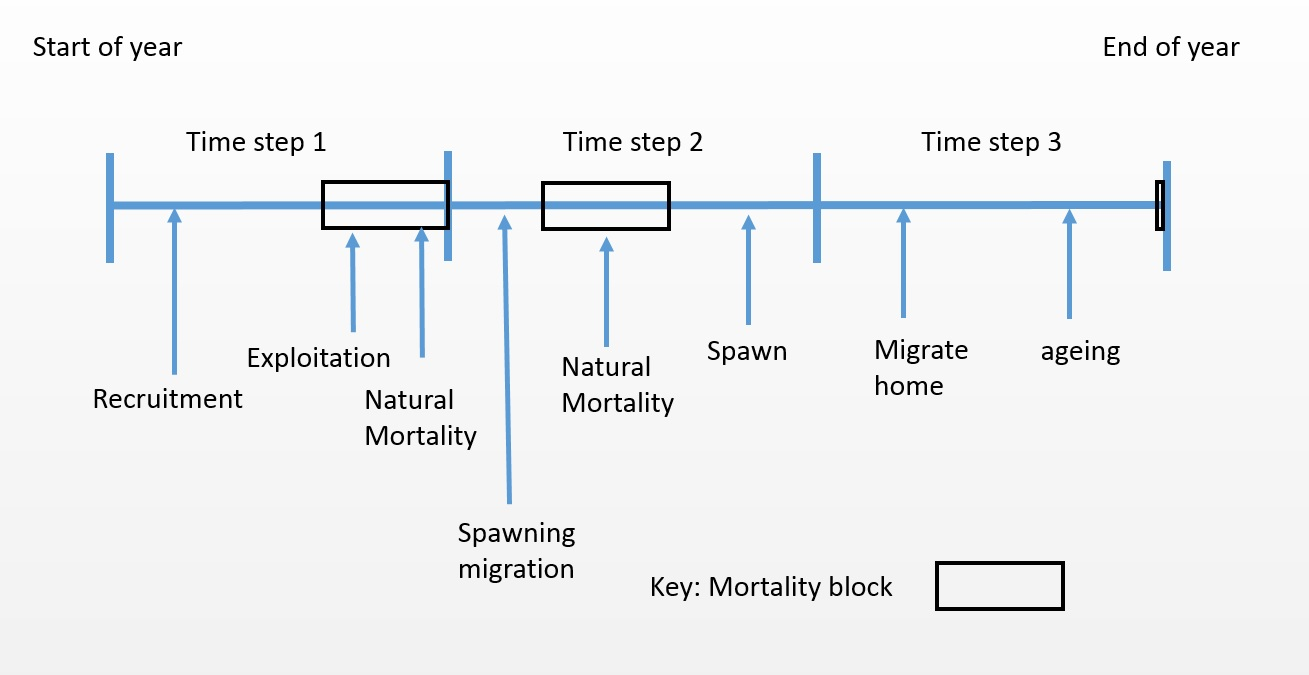
\includegraphics[scale=0.5]{Figures/annual_cycle.jpg}
	\caption{A example sequence for an annual cycle for an age-based model.}\label{Fig:annual}
\end{figure}

This would be specified using \command{time\_step} block:

{\small{\begin{verbatim}
@model
time_steps step1 step2 step3
\end{verbatim}}}

This gives the order and labels for each time step, i.e., 3. Processes are sequenced using order within the \command{time\_step} block:

\ifAgeBased
{\small{\begin{verbatim}
@time_step step1
processes Recruitment Fishing

@time_step step2
processes Spawn_migration Fishing

@time_step step3
processes Home_migration Ageing
\end{verbatim}}}
\else
{\small{\begin{verbatim}
			@time_step step1
			processes Recruitment Fishing
			
			@time_step step2
			processes Spawn_migration Fishing
			
			@time_step step3
			processes Home_migration Growth
\end{verbatim}}}
\fi

The \emph{Recruitment}, \emph{Fishing}, \emph{Spawn\_migration}, \emph{Home\_migration} and \ifAgeBased \emph{Ageing} \else \emph{Growth} \fi are all labels of command blocks that defines a process (see Section \ref{sec:Process} for the list of available processes). The order that the  processes are executed is in the same order as specified. The process \emph{Fishing} could be the process type \texttt{Instantaneous\_Mortality} (Section \ref{sec:Process-MortalityInstantaneous}) which takes natural mortality as a parameter as well as specifying the catches in the time-steps, so it is possible to have all catch taken in time-step \emph{step1} with some natural mortality, and no fishing in time-step \emph{step2} where the rest of the natural mortality occurs.

Although the process \emph{Spawn} represents a biological process, spawning, in the \CNAME\ model it is the time that the spawning stock biomass ($SSB$) is calculated since this is needed to calculate recruitment if there is a spawner-recruitment relationship. A related concept is maturity which can be in the partition, so there needs to be a process to transfer immature fish into the mature category, but it is only indirectly related to spawning. Hence, in modelling, spawning is not a process that affects the partition directly, but it the time to calculate the $SSB$ which must be defined as a derived quantity (from the partition). Hence, \emph{Spawn} is located in Figure \ref{Fig:annual}.

To calculate the $SSB$ a \command{derived\_quantity} command block is needed in which the "timing" of the $SSB$ calculation in terms of which time-step and the proportion of natural mortality within it is specified (\ref{sec:DerivedQuantity}).

\subsubsection{\I{The initialisation phases}}\label{sec:Initialisation}

Initialisation is the process of determining the model starting state at the start of the first year (\texttt{Start\_year}. The initial state can be equilibrium/steady state or some other initial state for the model (e.g., exploited), prior to the start year of the model.

There are multiple options for partition initialisation in \CNAME, including

\begin{itemize}
	\item Iterative: run the model for a specified number of years to get the converged state.
	\item Derived: Use the analytical solution (i.e., faster than iterative) for the initial state, but it does not work with some processes (e.g., density-dependent migration)
	\ifAgeBased
	\item Cinitial: Estimate the initial partition's numbers-at-age
	\item state\_category\_by\_age: specify the partition's numbers-at-age
	\else
	%\item Cinitial: Estimate the initial partition's numbers-at-length
    %\item state\_category\_by\_length: specify the partition's numbers-at-length
    \fi
\end{itemize}

Initialisation definitions start with specifying the initialisation label in the \command{model} command block followed by a \command{initialisation\_phase} command block specifying the type and other settings:

{\small{\begin{verbatim}
@model
...     # other subcommands
initialisation_phase int_label

@initialisation_phase int_label
type iterative  #choose one from the list above
...             # specify option values

\end{verbatim}}}

If needed, the processes used and their order in the initialisation are those specified in the annual cycle, but these can by changed by either excluding some processes or including others by using the  \texttt{exclude\_processes} or  \texttt{insert\_processes} subcommands in the \textit{initialisation\_phase} command blocks,

{\small{\begin{verbatim}

@initialisation_phase int_label
type iterative
exclude_processes Fishing
insert_processes step1(recruitment)=initialFishing
            # format: <step>(<insert before process label>)=<new block label>
...         # specify option values

\end{verbatim}}}

where \textit{Fishing} is the normal fishing process which defines natural mortality so when excluded, initialisation can use another value that incorporates some unrecorded fishing before the start of the assessment period by setting natural mortality to a higher value in the process \textit{initialFishing}. The place to insert \textit{initialFishing} is in the time-step labelled \textit{step1} before the process \textit{recruitment} which must be in that time-step (process label is enclosed in brackets). To insert at the end of the time-step use \textit{()}, e.g. \textit{step1()=initialFishing}.

For most models the most common type of initialisation phase to define an initial equilibrium age structure is \subcommand{derived}, whereas for length-based models the only type available is \subcommand{iterative}. Additional initialisation phases can be included by sequencing other phases one after another

{\small{\begin{verbatim}
@model
...     # other subcommands
initialisation_phase int_label int_label2


@initialisation_phase int_label
type derived    #choose one from the list above
...             # specify option values

@initialisation_phase int_label2
type iterative    #choose one from the list above
...             # specify option values

\end{verbatim}}}

which may be faster overall since fewer iterations may be required used in the second phase. The order of applying each initialisation is that given in the \command{model} command block.

The multi-phased initialisation allows for flexibility in the number and type of initialisation processes, for initialising a non-equilibrium starting state, or applying simple processes before applying more complex ones.

In each initialisation phase, the processes defined for that phase are applied and used as the starting point for the following phase or, if it is the last phase, the start year of the model.

The \emph{first} initialisation phase is always initialised with each \ifAgeBased age \else length class \fi and category set to zero. Care must be taken when using complex category inter-relationships or density-dependent processes that depend on a previously calculated state, as they may fail when used in the first phase of an initialisation.

Multi-phase iterations\index{Multi-phase iteration} can also be used to determine if an initialisation has converged. A second initialisation phase can be added for 1 year, with the same processes applied as in the first phase. The state at the end of the first and second phase is then output. If these states are identical, then it is likely that the initialisation has converged to an equilibrium state.

For multi-phase initialisation models, it is advised to include the \command{report} of type \subcommand{initialisation\_partition}. This will print the partition at the end of each initialisation phase, which can be useful for assessing the impact of each phase on the partition.

{\small{\begin{verbatim}
@report initial_partitions
type initialisation_partition
\end{verbatim}}}

\paragraph{\I{Iterative Initialisation}}\label{sec:InitialisationPhase-Iterative}

The \subcommand{iterative} initialisation is a general solution for initialising the model, but can be slow to converge, depending on the model. Its value is that it can work on complex structured models that may be difficult or impossible to implement using analytic approximations.

The number of iterations in the iterative initialisation can increase the model output, and the number of iterations should be chosen to be large enough to allow the population state to fully converge. In an age-based model, a period of about two times the maximum age is recommended to ensure convergence. In length-based models a longer time may be required depending on the nature of the growth increment process. \CNAME\ can report a convergence statistic to assist in determining if adequate convergence has been obtained.

In addition, the iterative initialisation phase can optionally be stopped early if the user-defined convergence criteria is met. For a list of supplied years in the initialisation phase, the convergence criteria is met if the proportional absolute summed difference between the state in year $t-1$ and the state in year $t$ ($\widehat{\lambda}$) is less than the user-defined value of $\lambda$, where

\begin{equation}
  \widehat{\lambda} = \frac{\sum\limits_{i,j}  \left|\text{element}(t)_{i,j} - \text{element}(t-1)_{i,j} \right|}{\sum\limits_{i,j} \frac{}{}\text{element}(t)_{i,j}}
\end{equation}

where $\text{element}(t)_{i,j}$ denotes the numbers at time step $t$ in category $j$ and \ifAgeBased age \else length class \fi $i$.

Hence, for the initialisation define:

\begin{itemize}
  \item The number of initialisation phases,
  \item The number of years in each phase, and
  \item The processes to apply in each phase, where the default processes are those applied in the annual cycle.
\end{itemize}

An example with one initialisation phase:

{\small{\begin{verbatim}
@model
...
initialisation_phases Iterative_initialisation

@initialisation_phase Iterative_initialisation
type iterative
years 50                # do 50 annual cycle iterations
lambda 0.0001
convergence_years 20 40 # test for convergence at 20 and 40 iterations
\end{verbatim}}}

A report on the outcome of the iterative convergence evaluation is available (\command{report} of type \subcommand{initialisation}). This will print the years when convergence was tested and the result of the convergence tests.

\ifAgeBased
\paragraph{\I{Derived Initialisation}}\label{sec:InitialisationPhase-Derived}

The \subcommand{derived} initialisation is an analytical solution that calculates the equilibrium age structure and the plus group using a geometric series solution. The benefit of this method is it can be solved in \texttt{max\_age - min\_age + 1} years or time-steps units, so it is computationally faster than the iterative initialisation phase. Under some process combinations (e.g., one-way migrations) this initialisation does not calculate the exact equilibrium partition. When using this initialisation, users can confirm that the plus group has reached an equilibrium state by either comparing with an iterative initialisation, or by adding a second iterative initialisation phase with a limited number of iterations for comparison.

An example with one initialisation phase:

{\small{\begin{verbatim}
		@model
		...
		initialisation_phases Equilibrium_initialisation

		@initialisation_phase Equilibrium_initialisation
		type derived
\end{verbatim}}}
\fi

When a model is initialised with \subcommand{derived} (for age-based models only) or \subcommand{iterative} (for either age-based or length-based models),  and recruitment is defined by \(B_0\), the model initialises the partition with \(R_0 = 1\). Once the initialisation phase is complete, it scales all the categories defined in each recruitment process by
\[
N_{a,c}  = N_{a,c} \times B_0^R / SSB^R  \ .
\]
where, \(R\) denotes each recruitment block and \(N_{a,c}\) are categories defined in that recruitment block. For this case, it is advised to associate all categories to the recruitment so they are accounted for in this scaling process. If maturity is in the partition, it is not intuitive, but they must be defined in the recruitment dynamic with a proportion set = 0 (for more information on specifying this see Section 
\ifAgeBased \ref{sec:Process-Recruitment} \else \ref{sec:Process-Recruitment} \fi). \CNAME\ will flag a warning if a model doesn't have all categories defined in the available recruitment blocks. A case where this can be ignored is in models with tagged categories, these categories don't exist during initialisation and so don't need to be scaled, and thus can be omitted from the recruitment definition. \CNAME\ will still output a warning for this, but can be ignored if users understand its purpose.

\ifAgeBased
\paragraph{\I{Cinitial Initialisation}}\label{sec:InitialisationPhase-Cinitial} \STATUS{Untested}

The \subcommand{cinitial} initialisation can only be applied after \subcommand{derived} or \subcommand{iterative} initialisation phases. This initialisation can be a method for estimating the non-equilibrium state of population if there is exploitation before observations are collected. The estimated \subcommand{cinitial} factors shift the initial population away from an equilibrium state prior to the start year.

After the first initialisation phase we have an equilibrium age-structure denoted by $N_{equil}$.

\subcommand{Ciniital} specifies an age structure denoted by $N_{cinit}$ (in numbers), but this can be combinations of categories, for example, both sexes by two areas.

$Multiplier =  N_{cinit} / N_{equil}^{combined}$

where $N_{equil}^{combined} $ is summed over the same combined categories as \textit{Cinitial}. Then

$N_{init} =  N_{equil} * Multiplier $

$N_{init}$ is the numbers-at-age by category for the start of the model run.

It would be helpful to include an observation of age composition data for the first year of the model in order to estimate the non-equilibrium population state.

An example with two initialisation phases:

{\small{\begin{verbatim}
		@model
		...
		initialisation_phases Iterative Cinitial

		@initialisation_phase Iterative
		type iterative
		years 10
		lambda 0.0001
		convergence_years 10 20

		@initialisation_phase Cinitial
		type cinitial
		categories spawn.male+nonspawn.male spawn.female+nonspawn.female
		table n
		spawn.male+nonspawn.male     5e7 5e7 7e6 6e6 5e6 4e6 3e6 2e6 1e6 1e6 1e1 1e1 1e1 1e1
		spawn.female+nonspawn.female 5e7 5e7 7e6 6e6 5e6 4e6 3e6 2e6 1e6 1e6 1e1 1e1 1e1 1e1
		end_table
		\end{verbatim}}}

The Cinitial factors can also be estimated with the syntax

{\small{\begin{verbatim}
	@estimate cinit_male
	parameter initialisation_phase[Cinitial].spawn.male+nonspawn.male
	same initialisation_phase[Cinitial].spawn.female+nonspawn.female
	lower_bound  2e2  2e2  2e2  2e2  2e2  2e2  2e2  2e2  2e2  2e2  2e0  2e0  2e0  2e0
	upper_bound  2e9  2e9  2e9  2e9  2e9  2e9  2e9  2e9  2e9  2e9  2e9  2e9  2e9  2e9
	type uniform
	\end{verbatim}}}

\paragraph{\I{State\_category\_by\_age}}\label{sec:InitialisationPhase-StateCategoryByAge}\label{sec:Process-LoadPartition}

The \subcommand{state\_category\_by\_age} initialisation uses a user-defined table as the initial partition numbers-at-age for the beginning of the  start year. Models can be initialised by specifying the numbers-at-age for each category.

An example with one initialisation phase:

{\small{\begin{verbatim}
		@model
		...
		initialisation_phases Fixed

		@initialisation_phase Fixed
		type state_category_by_age
		categories male female
		min_age 3
		max_age 10
		table n
		male   1000 900 800 700 600 500 400 700
		female 1000 900 800 700 600 500 400 700
		end_table
		\end{verbatim}}}

When initialising models with this type, undefined behaviour may result if the model applies processes that require derived quantities to be calculated in the initialisation phase. (e.g., $SSB$ so that recruitment can be calculated for the start year). In the latter case, the user would have to use a subsequent initialisation phase \subcommand{iterative} that has natural mortality set to zero (i.e., \subcommand{insert\_processes} subcommand to introduce zero natural mortality and \subcommand{exclude\_processes} to exclude the mortality process that defines natural mortality) for as many year needed to calculate the $SSB$ values.

\subsubsection{\I{Non-equilibrium initialisation phases}}\label{sec:Initialisation-NonEquilibrium}

This section provides tips and advice for configuring \CNAME\ models to have non-equilibrium age or length structures at the model \subcommand{start\_year}. An equilibrium age or length structure in this context, roughly refers to an age-structure that would result if the annual cycle was repeatedly run with no fishing. For many models this will result in an age or length structure that has an exponential decay from natural mortality and constant recruitment.

As mentioned in the above section, the \subcommand{cinitial} initialisation type can be used to after either \subcommand{derived} or \subcommand{iterative} to produce a non-equilibrium age structure. However, recent simulations have shown difficulties in estimating the parameters from this phase \citep{roberts_dunn_estimate_start_M_init}. Another approach also explored by \cite{roberts_dunn_estimate_start_M_init}, was to start the model \subcommand{max\_age} years before the intended \subcommand{start\_year} and estimate additional recruitment parameters during this phase so that by the intended \subcommand{start\_year}, the age structure would be in a non-equilibrium state.
\fi % currently these are only availble in age-based models.

\ifAgeBased
Another approach that is similar to the \subcommand{cinitial} initialisation type is to first run either \subcommand{derived} or \subcommand{iterative} phase and then to apply a second \subcommand{iterative} phase that has an additional initialisation mortality process.

There are a range of mortality processes that can only be applied during initialisation. These are

\begin{itemize}
	\item \subcommand{mortality\_initialisation\_event} see Section~\ref{sec:Process-MortalityInitialisationEvent}
	\item \subcommand{mortality\_initialisation\_event\_biomass} see Section~\ref{sec:Process-MortalityInitialisationEventBiomass}
	\item \subcommand{mortality\_initialisation\_baranov} see  Section~\ref{sec:Process-MortalityInitialisationBaranov}
\end{itemize}
\fi % end if

\subsection{\I{Population processes}}\label{sec:Process}

\ifAgeBased

Population processes are processes that change the model state. These processes produce changes in the partition by adding or removing individuals, or by moving individuals between ages and/or categories.

Current population processes available include:

\begin{itemize}
\item recruitment\index{Recruitment} (Section~\ref{sec:Process-Recruitment}),
\item ageing\index{Ageing} (Section~\ref{sec:Process-Ageing}),
\item growth\index{Growth} (Section~\ref{sec:AgeLength}),
\item maturation\index{Maturation} (Section~\ref{sec:Process-TransitionCategory}),
\item mortality\index{Mortality} events (e.g., natural and fishing) (Section~\ref{sec:Process-Mortality}), 
\item category transition processes\index{Category transition}, i.e., processes that move individuals between categories while preserving their overall age structure (Section~\ref{sec:Process-TransitionCategory}), and
\item tagging and tag loss (Section~\ref{sec:Process-TagByAge}).
\end{itemize}

There are two types of processes: (1) processes that occur across multiple time steps in the annual cycle, e.g., \subcommand{mortality\_constant\_rate} and \subcommand{mortality\_instantaneous}; and (2) processes that occur only within the time step in which they are specified.

\subsubsection{\I{Recruitment}}\label{sec:Process-Recruitment}

Recruitment processes  add new individuals to the partition. Recruitment depends on virgin biomass or alternatively recruitment in the virgin state and so these parameters are located in this process (as \textit{b0} and \textit{r0}). The other factors needed are SSB if there is a stock-recruitment relationship and the CV for the prior on YCS (the mean is mandated to be 1 over some specified year range). Thus, a SSB label may have to be included (pointing to a derived quantity).

In the recruitment processes, a number of individuals are added to a single age class (subcommand \textit{age}) within the partition, with the number determined by the type of stock-recruitment process specified. If recruits are added to more than one category, then the proportion of recruits to be added to each category is specified by the \argument{proportions} subcommand. For example, if recruiting to categories labelled \texttt{male} and \texttt{female}, then the proportions may be set to $0.5$ and $0.5$, so that half of the recruits are added to the male category and the other half to the female category.

Recruitment can differ between a spawning event or the creation of a cohort/year class. One view for fisheries is that recruitment usually refers to individuals "recruiting" to a fishery. This definition is used because there is usually not a lot of information on younger age classes between the time of spawning and being vulnerable to a survey or fishery for data collection. However, here, recruitment is to a fixed age class for one or more categories.

The offset between spawning and recruitment is parametrised either by the recruitment subcommand \texttt{age}, or \texttt{min\_age}, which is the default value for the \texttt{age} subcommand in the recruitment process. The \CNAME\ parameter \texttt{age} is the same as the CASAL parameter \texttt{y\_enter}.\TODO{Check this} Notice that the minimum age is usually different from zero and so there is usually  a one or more year's delay between spawning and recruitment into the partition. There is also a complication from when spawning occurs in the annual cycle and when recruitment occurs.

\CNAME\ has two  recruitment processes, constant recruitment\index{Recruitment ! Constant} and the \I{Beverton-Holt stock-recruitment relationship}\index{Recruitment ! Beverton-Holt} \citep{1203}. The  number of individuals following recruitment in year $y$ is

\begin{equation}
N_{y,a,j} \leftarrow N_{y,a - 1,j} + p_j(R_y)
\end{equation}

where $N_{y,a,j}$ is the numbers in year $y$ and category $j$ at age $a$, $p_j$ is the proportion added to category $j$, and $R_y$ is the total number of recruits in year $y$.

\paragraph{\I{Constant recruitment}}\label{sec:Process-RecruitmentConstant}

In the constant recruitment process the total number of recruits added in each year $y$ in age $a$ is $R_y$, with $R_y = R_0$ for all years

\begin{equation}
  R_{y,j} = p_j(R_0)
\end{equation}

Constant recruitment is equivalent to a Beverton-Holt recruitment process with steepness ($h$) set to 1.

For example, to specify a constant recruitment process where individuals are added to the male and female immature categories at $age=1$ in equal proportion (\texttt{proportions} = 0.5), and the number to add is $R_0=5 \times 10^5$, the syntax is

{\small{\begin{verbatim}
	@process Recruitment
	type constant_recruitment
	categories male.immature female.immature
	proportions 0.5 0.5
	r0 500000
	age 1
\end{verbatim}}}

\paragraph{\I{Beverton-Holt recruitment}}\label{sec:Process-RecruitmentBevertonHolt}

In the Beverton-Holt recruitment process the total number of recruits added each year is $R_y$. $R_y$ is the product of the average recruitment $R_0$, the annual year class strength multiplier $YCS$, and the stock-recruit relationship $SR(SSB_y)$

\begin{equation}\label{eq:BH}
  R_{y,a,j} = p_j(R_0 \times YCS_{ycs\_year} \times SR(SSB_{ycs\_year}))
\end{equation}

where

\begin{equation}\label{eq:year_class}
ycs\_year = y - \texttt{ssb\_offset}
\end{equation}

and $a$ is age, $p_j$ is the proportion of recruits to enter category $j$, and \texttt{ssb\_offset} is the number of years lag between spawning and recruitment.

Recruitment refers to recruitment into the population and may differ from the spawning event. See below on more information about \texttt{ssb\_offset}. In general this parameter should not be specified by the user.

$SR(SSB_y)$ is the Beverton-Holt stock-recruit relationship parametrised by the steepness $h$, and based on \cite{mace_doonan_88} parametrisation

\begin{equation}\label{eq:BH_SR}
SR(SSB_y) = \frac{SSB_y}{B_0} / \left( 1-\frac{5h-1}{4h} \left( 1-\frac{SSB_y}{B_0} \right) \right)
\end{equation}

The Beverton-Holt recruitment process requires a value for \Bzero\ and $SSB_y$ to calculate the number of recruits. A derived quantity (see Section \ref{sec:DerivedQuantity}) must be defined that provides the annual $SSB_y$ for the recruitment process. \Bzero\ is then defined as the value of the $SSB$ at the end of one of the initialisation phases, which is defined by the parameter \texttt{b0\_initialisation\_phase}.

During initialisation the $YCS$ multipliers are assumed to be equal to 1, and recruitment that happens in the initialisation phases that occur before and during the phase when \Bzero\ is determined are assumed to have steepness $h=1$ (i.e., in those initialisation phases, recruitment is equal to \Rzero).

Recruitment in the initialisation phases after the phase where \Bzero\ was determined are calculated using the Beverton-Holt stock-recruit relationship. \Rzero\ and \Bzero\ have a direct relationship when there are no density-dependent processes in the annual cycle. Models can thus be initialised using \Bzero\ or \Rzero.

An example of the specification of a Beverton-Holt recruitment process, where individuals are added to the category "immature" at $age=1$, and the number added is $R_0=5 \times 10^5$; \texttt{SSB\_derived\_quantity} is a derived quantity that specifies the total spawning stock biomass that contributed to the year class, with \Bzero\ the value of the derived quantity at the end of the initialisation phase labelled \texttt{phase1}; and $YCS$ are standardised to have mean one in the period 1995 to 2004, and recruits enter into the model two years following spawning

{\small{\begin{verbatim}
	@process Recruitment
	type recruitment_beverton_holt
	categories immature
	proportions 1.0
	r0 500000
	b0_initialisation_phase phase1
	steepness 0.75
	age 1
	ssb SSB_derived_quantity

\end{verbatim}}}

The property \texttt{ssb\_offset} should not be manually specified; \CNAME\ determines \texttt{ssb\_offset} by the order of ageing, recruitment, spawning, and the recruitment parameter \texttt{age}

\begin{itemize}
	\item if the annual time step order is recruitment, ageing, spawning, then \texttt{ssb\_offset} should equal \texttt{age} + 1, or
	\item if the annual time step order is spawning, ageing, recruitment, then \texttt{ssb\_offset} should equal \texttt{age} - 1, or
	\item \texttt{ssb\_offset} = \texttt{age}
\end{itemize}

There may be scenarios where the user will input these values, e.g., if there are multiple ageing processes in the annual cycle. \CNAME\ does not have functionality to accommodate this situation, so in this case \texttt{ssb\_offset} would be manually defined.

There are two variants of this process and they refer to how the stock recruitment residuals or $YCS_{ycs\_year}$ are parametrised. This parametrisation can either be in natural space as year class strength ($YCS$) multipliers, or in log space as recruitment deviations. Due to the difference in terminology, these variants are implemented in two separate processes, \subcommand{type recruitment\_beverton\_holt} and \subcommand{type recruitment\_beverton\_holt\_with\_deviations}, respectively.

\paragraph*{YCS ($YCS_y$)}

The $YCS$ parameter (\texttt{ycs\_years}) is defined in Equation~\eqref{eq:year_class}. The parameter \texttt{ycs\_values} is referenced by the \texttt{ycs\_years} parameter and is important to note when defining \command{estimate}, \command{project}, and \command{time\_varying} blocks for the parameter \texttt{ycs\_values}. An example is at the end of the section.

A common practice when estimating $YCS$ is to standardise using the Haist parametrisation, which was described by V. Haist. \CNAME\ will standardise $YCS$ only if subcommand \subcommand{standardise\_ycs\_years} is defined. The model parameter \texttt{ycs\_values} is a vector \textbf{Y}, covering the years from \texttt{start\_year} - \texttt{ssb\_offset} to \texttt{final\_year} - \texttt{ssb\_offset}, as defined by the parameter \texttt{ycs\_years}. The resulting year class strengths are calculated by $YCS_i=Y_i/\bar{\textbf{Y}}$, where the mean is calculated over the user-specified years \texttt{standardise\_ycs\_years}.

An alternative to \enquote{standardisation} is to constrain the $YCS$ parameters using the simplex transformation (see Section~\ref{sec:Transformation-Simplex}). This is thought to have estimation benefits over the \enquote{standardisation} as priors can be applied to the \enquote{free} parameters (\(Y_i\)).

\[
YCS_i =
\begin{cases}
Y_i / mean_{y \in S}(Y_y) & :y \in S\\
Y_i					 & :y \notin S
\end{cases}
\]

where S is the set of years from \texttt{standardise\_ycs\_years}. One effect of this parametrisation is that \Rzero\ is then defined as the mean estimated recruitment over the set of years $S$, because the mean $YCS$ multiplier over these years will always be one.

Typically \texttt{standardise\_ycs\_years} is defined to span the years over which $YCS$ is reasonably well estimated. For years that are not well estimated, $Y_y$ can be set to 1 for some or all years $y\in S$ (which is equivalent to forcing $R_y$ = \Rzero\ x $SR(SSB_y)$) by setting the lower and upper bounds of these $Y$ values to 1. An exception to this might occur for the most recent $YCS$ values, which the user may estimate but not include in the definition of \Rzero\ (because the estimates may be based on too few data). One or more years may be excluded from the range of years for the averaging process of the Haist parametrisation.

The advantage of the Haist parametrisation is that a large penalty is not necessary to force the mean of the $YCS$ parameter to be 1, although a small penalty should still be used to stop the mean of \textbf{Y} from drifting. These adjustments may improve MCMC performance. Projected $YCS$ values are not affected by this feature. A disadvantage with this parametrisation in a Bayesian analysis is that the prior applies to $Y$, not $YCS$.

In the  example given above,  $YCS$ are standardised to have mean one in the period 1995 to 2004, and recruits enter into the model two years following spawning

{\small{\begin{verbatim}
	@process Recruitment
	type recruitment_beverton_holt
	...            #subcommand above
	standardise_ycs_years 1995:2004
	ycs_years  1994 1995 1996 1997 1998 1999 2000 2001 2002 2003 2004 2005 2006
	ycs_values 0.65 0.87  1.6 1.13 1.02 0.38 2.65 1.35    1    1    1    1    1
\end{verbatim}}}


\paragraph*{Recruitment deviations, $\epsilon_y$ (\emph{type recruitment\_beverton\_holt\_with\_deviations})} \label{sec:Process-RecruitmentBevertonHoltWithDeviations} \STATUS{Untested}

Recruitment deviations represent the stock-recruitment relationship residuals in log space, with the link between $YCS_y$ and $\epsilon_y$

\begin{equation}\label{eq:recruit_devs}
	YCS_y = exp(\epsilon_y - b_y\sigma^2_R / 2)
\end{equation}

where $\epsilon_y\sim N(0,\sigma^2_R)$, $\sigma^2_R$ is the variance of the stock-recruitment residuals, and $b_y$ is a bias correction defined by \cite{methot2011adjusting}

\begin{equation}\label{eq::bias}
b_y = \left\{\begin{array}{lr}
0, & \text{for }y\leq y_1^b\\
b_{max}(1 - \frac{y - y_1^b}{y_2^b - y_1^b}), & \text{for } y_1^b < y < y_2^b\\
b_{max}, & \text{for } y_2^b\leq y \leq y_3^b\\
b_{max}(1 - \frac{y_3^b - y}{y_4^b - y_3^b}), & \text{for }  y_3^b< y < y_4^b\\
0, & \text{for } y_4^b\leq y
\end{array}\right\}
\end{equation}

The $\epsilon_y$ values are normally distributed in log space and thus lognormal when back-transformed to the resulting stock-recruitment relationship $YCS_y$. Recent work has found that this transformation does not technically lead to the \textit{a priori} assumption that the resulting $YCS_y$ are lognormal. \TODO{See Appendix investigating-two-options-for-ycs-prior-distribution-formulations for more details.}

The ramp function described above for the bias correction has the additional subcommands controlling the ramp

\begin{itemize}
	\item $y_1^b = $ \subcommand{last\_year\_with\_no\_bias}
	\item $y_2^b = $ \subcommand{first\_year\_with\_bias}
	\item $y_3^b = $ \subcommand{last\_year\_with\_bias}
	\item $y_4^b = $ \subcommand{first\_recent\_year\_with\_no\_bias}
	\item $b_{max} = $ \subcommand{b\_max}
\end{itemize}

{\small{\begin{verbatim}
@process Recruitment
type recruitment_beverton_holt_with_deviations
categories immature
proportions 1.0
r0 500000
last_year_with_no_bias 1940
first_year_with_bias 1950
last_year_with_bias 2016
first_recent_year_with_no_bias 2018
b_max 0.85
b0_initialisation_phase phase1
steepness 0.75
age 1
ssb SSB_derived_quantity
deviation_years  1994-2006
deviation_values 0 -0.2 0.4 0 0 0 0 0 0 0 0 0 0
\end{verbatim}}}

\paragraph*{Recruitment when modelling two stocks (or species)}

To specify a Beverton-Holt recruitment for each stock, the information required is:

\begin{enumerate}
	\item $YCS$, starting from year (\texttt{start\_year} - \texttt{ssb\_offset}) and extending up to year (\texttt{final\_year} - \texttt{ssb\_offset})
	\item the value of \texttt{age} (which is \texttt{y\_enter} in CASAL)
	\item the steepness parameter \texttt{h}
	\item in a multi category model, the proportion of recruits for each category
	\item a label for the derived quantity
\end{enumerate}

When an \command{initialisation\_phase} (Section~\ref{sec:Initialisation}) type = \subcommand{derived} is specified and the recruitment is defined by \subcommand{b0}, then all categories must be specified in the \command{recruitment} block. Usually in a recruitment processes only the categories that receive recruits need to be defined. For example, a population has a spawning area that is different from the area where recruits enter the population. An area-specific model could then be specified which contains spawning categories and recruiting categories. The recruiting categories would be specified in the subcommand \subcommand{categories}, as these would be the categories receiving recruits.

If \command{initialisation\_phase}, \subcommand{type=derived} is used, then all categories that are a part of that recruitment process need to be specified as well. For example,

{\small{\begin{verbatim}
@process Recruitment_stock1
type recruitment_beverton_holt
categories stock1.immature.M stock1.immature.female stock1.spawn.male stock1.spawn.female
proportions 0.5 0.5 0.0 0.0
r0 500000
ssb SSB1
....
\end{verbatim}}}

{\small{\begin{verbatim}
@process Recruitment_stock2
type recruitment_beverton_holt
categories stock2.immature.male stock2.immature.female stock2.spawn.male stock2.spawn.female
proportions 0.5 0.5 0.0 0.0
r0 200000
ssb SSB2
....
\end{verbatim}}}

The \texttt{proportions = 0.0} for "spawn.male" and "spawn.female" are needed due to the way the derived initialisation phase works. The derived initialisation finds a solution for when \subcommand{r0} = 1.0 based on an infinite geometric series for the plus group, and scales the initial partition by \subcommand{r0}. Thus, if all categories are not specified, then those that are missed would not be initialised to true values and this could lead to inaccurate model outputs. This set-up extends to multiple-stock fisheries model configurations as well, where all of the categories that make up the stock need to be listed.

\subsubsection{\I{Ageing}\label{sec:Process-Ageing}}

The ageing process "ages" individuals, i.e., this process moves all individuals in the named categories $j$ from one age class $a$ to age class $a + 1$, or accumulates them if the last age class is a plus group.

The ageing process is defined as,
\begin{equation}
  \text{element}(a + 1,j) \leftarrow \text{element}(a,j)
\end{equation}

except in the case of the plus group (if defined),
\begin{equation}
  \text{element}(a_{\text{max}}, j) \leftarrow \text{element}(a_{\text{max}}, j) + \text{element}(a_{\text{max}-1}, j).
\end{equation}

For example, to apply ageing to the categories \texttt{immature} and \texttt{mature}, the syntax is

{\small{\begin{verbatim}
	@process Ageing
	type ageing
	categories immature mature
	\end{verbatim}}}

Note: the ageing process is \emph{NOT} applied by \CNAME\ by default --- it needs to be explicitly specified. As with all other processes, \CNAME\ will not apply a process unless it is defined and specified within the annual cycle. Hence, it is possible to specify a model where a category is not aged. \emph{\CNAME\ will not check or otherwise warn if there is a category defined where ageing is not applied.}

\subsubsection{\I{Mortality}\label{sec:Process-Mortality}}

There are 8 types of mortality processes available in \CNAME, and three tag related processes that also cause mortality:

\begin{itemize}
	\item constant rate,
	\item event,
	\item biomass-event,
	\item instantaneous,
	\item instantaneous retained (discards),
	\item Holling,
	\item initialisation, and
	\item a density-dependent relationship based on prey suitability.
	\item Tag-release by age
	\item Tag-release by length	
	\item Tag-loss
\end{itemize}

These processes remove individuals from the partition, either as a rate, as a total number (abundance), as a biomass of individuals or, as a combination of these. \CNAME\ does not (yet) implement the Baranov catch equation. However, instantaneous mortality is considered an approximation to the Baranov catch equation.

To apply both natural and biomass-event mortality, the mortality type \texttt{mortality\_instantaneous} can be specified. Or, you can use \texttt{mortality\_instantaneous\_retained}, where discards are allowed. Mortality blocks are special because they allow both natural mortality and fishing mortality at the same time. Note that all mortality processes occur within the mortality block of a time step. See Section~\ref{sec:MortalityBlock} for more information and definitions on mortality blocks.


\paragraph{\I{Timing evaluation interval; timing the point when observations are fitted or derived quantities are evaluated }}\label{sec:MortalityBlock}\label{sec:TimingEvaluationInterval}

\TODO{review; put into observations?}

Observations (see Section~\ref{sec:Observation})  and derived quantities (see Section~\ref{sec:DerivedQuantity}) need a concept called a \emph{timing evaluation interval} so that the "time" within a year can be specified for their fit or evaluation. This interval is intimately tied into mortality processes.

There can be one or more mortality processes specified within a time-step, but these must be grouped sequentially, i.e., there cannot be a non-mortality process between any two mortality processes within any one time step. The sequence of mortality processes is called a \emph{timing evaluation interval}. If no mortality processes occurs in a time step, then the \emph{timing evaluation interval} is defined to occur at the end of the time step, i.e., it is a virtual, unspecified,  process. Thus  each time step has one \emph{timing evaluation interval}.

\CNAME\ will output an error if more than one \textit{timing evaluation interval} occurs in a single time step.

The "time" for an observation or derived quantity is based on the proportion of mortality that has occurred within the \textit{timing evaluation interval}. The starting and ending partition are saved so that a partition can be estimated by  interpolation between the start and end partitions.

For example, the point of calculation can be set to a point  when 75 \% of the deaths from natural mortality plus catch has occurred The partition at this point is based on interpolating between the start and end of the interval as the partition is known at those points.  Two  methods are available: \texttt{weighted\_sum} and \texttt{weighted\_product}, and are defined as

\begin{itemize}
	\item \texttt{weighted\_sum}: after proportion $p$ through the mortality block, the partition elements are given by $n_{p,j} = (1 - p)n_j + p'_j$

	\item \texttt{weighted\_product}: after proportion $p$ through the mortality block, the partition elements are given by $n_{p,j} = n_j^{1-p} n'^p_j$
\end{itemize}

where $n_{p,j}$ is the derived quantity at proportion $p$ of the mortality block for category $j$, $n_j$ is the quantity at the beginning of the mortality block, and $n'_j$ is the quantity at the end of the mortality block.

In the case of a virtual \textit{timing evaluation interval}, the partition at the end of the time-step is used.

\TODO{REDO FIGURE TO REFLECT TEI rather than mortality blocks; have two mortality processes in step 2}

\begin{figure}[H]
	\centering
	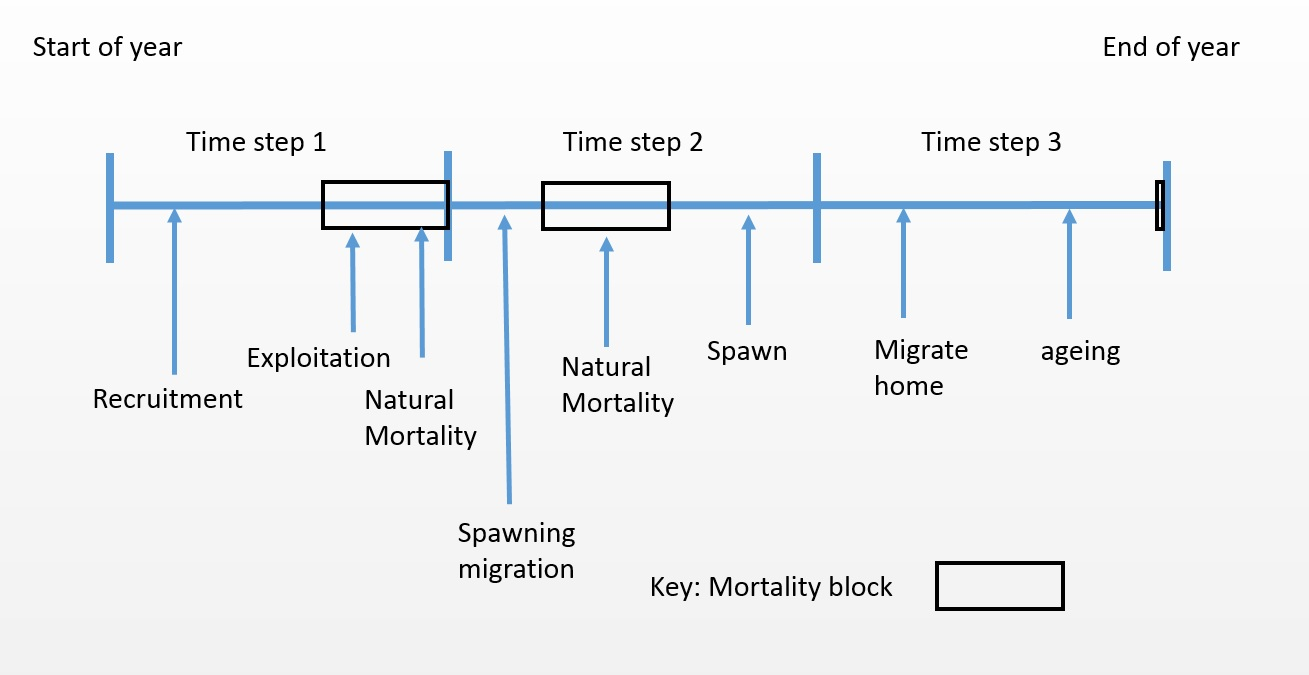
\includegraphics[scale=0.5]{Figures/annual_cycle.jpg}
	\caption{A example sequence for an annual cycle.}\label{Fig:annual2}
\end{figure}


\TODO{GO OVER M and specifying M-by-age HERE FOR ALL M-BASED PROCESSES}
\TODO{MAX U rate specification + Penalities}

\paragraph{Constant mortality rate}\label{sec:Process-MortalityConstantRate} 

To specify a constant annual mortality rate \index{Constant mortality}(e.g. $M=0.2$) for categories "male" and "female"

{\small{\begin{verbatim}
# A process with label NaturalMortality
@process NaturalMortality
type          mortality_constant_rate
categories    male female
# effectively age related mortality
relative_m_by_age One One
m             0.2 0.2
\end{verbatim}}}

The total number of individuals removed from a category

\begin{equation}
D_{j,t} = \sum_a N_{a,j,t} [1 - \exp(-S_{a,j} M_{a,j} p_t)]
\end{equation}

where $D_{j,t}$ is the total number of deaths in category $j$ in time step $t$, $N_{a,j,t}$ is the number of individuals in category $j$ of age $a$ in time step $t$, $S_{a,j}$ is the selectivity value for age $a$ in category $j$, $M_{a,j}$ is the mortality rate for category $j$ for age $a$, and $p_t$ is the proportion of the mortality rate to apply in time step $t$.

The mortality rate process requires the specification of the mortality-by-age curve which is specified using a selectivity. To apply the same mortality rate over all age classes in a category, use a selectivity defined as $S_{a,j}=1.0$ for all ages $a$ in category $j$

{\small{\begin{verbatim}
@selectivity One
type constant
c 1
\end{verbatim}}}

Age-specific mortality rates can also be applied. For example, the hypothesis that mortality is higher for younger and older individuals and lowest when individuals are at their optimal fitness could be defined by using a double exponential selectivity (see Section~\ref{sec:Selectivity})

{\small{\begin{verbatim}
@selectivity age_specific_M
type double_exponential
x0 7.06524
x1 1
x2 17
y0 0.182154
y1 1.43768
y2 1.57169
alpha 1.0

@process      NaturalMortalityByAge
type          mortality_constant_rate
categories    male female
relative_m_by_age age_specific_M age_specific_M
m             1.0 1.0
\end{verbatim}}}

\TODO{INSERT FIG OF M-by-age}

In this definition \subcommand{m} is set to 1.0 and the rate is described through the selectivity. Otherwise, $M_{age} = S_{age} * m$. This concept can be constructed similarly for other mortality methods such as \subcommand{instantaneous\_mortality}.

\paragraph{Event and biomass-event mortality}\label{sec:Process-MortalityEvent}\label{sec:Process-MortalityEventBiomass} \STATUS{Untested?}

\TODO{WHEN NOT DOING M and FISHING AT THE SAME TIME}

The event mortality\index{Event mortality} and biomass-event mortality\index{Biomass-event mortality} processes are applied in a similar manner, except that they remove a specified abundance (number of individuals) or biomass, respectively. These mortality processes can be used to define mortality events where the numbers of removals are known, e.g., fishing, rather than applying mortality as a rate.

In these cases, the abundance or biomass removed is also constrained by a maximum exploitation rate. \CNAME\ removes as many individuals or as much biomass as possible,  while not exceeding the maximum exploitation rate.

Event mortality processes require a penalty to avoid estimating parameter values that will not allow the defined number of individuals to be removed. The model penalises those parameter estimates that result in an too low a number of individuals in the defined categories (after applying selectivities) to allow for removals at the maximum exploitation rate, with a similar penalty for biomass. See Section \ref{sec:Penalty} for more information on how to specify penalties.

The event mortality applied to user-defined categories $i$, with the numbers removed at age $j$ determined by a selectivity-at-age $S_j$:

First, calculate the vulnerable abundance for each category $j$ in $1 \ldots J$ for ages $a = 1 \ldots A$ that are subject to event mortality

\begin{equation}
  V_{a,j} = S_{a,j} N_{a,j}
\end{equation}

and define the total vulnerable abundance $V_{total}$ as

\begin{equation}
  V_{total}  = \sum\limits_j {\sum\limits_a {V_{a,j}}}
\end{equation}

The exploitation rate\index{Maximum exploitation rate} to apply is

\begin{equation}
U = \begin{cases}
  C/V_{total}, & \text{if $C/V_{total} \leq U_{max}$} \\
  U_{max}, & \text{otherwise}\\
  \end{cases}
\end{equation}

The number removed $R_{a,j}$ from each age $a$ in category $j$ is,

\begin{equation}
  R_{a,j} = U V_{a,j}
\end{equation}

For example, to specify an \textbf{abundance-based} fishing mortality process with catches given for a set of specific years over categories "immature" and "mature", with selectivity "FishingSel", and assuming a maximum possible exploitation rate of 0.7, the syntax is

{\small{\begin{verbatim}
	@process     Fishing
	type          event_mortality
	categories    immature mature
	years         2000 2001 2002 2003
	U_max         0.70
	selectivities FishingSel FishingSel
	penalty       event_mortality_penalty
	\end{verbatim}}}

and specified similarly for a \textbf{biomass-based} fishing mortality process

{\small{\begin{verbatim}
		@process      Fishing
		type          mortality_event_biomass
		categories    immature mature
		years         2000 2001 2002 2003
		U_max         0.70
		selectivities FishingSel FishingSel
		penalty      event_mortality_penalty
		\end{verbatim}}}

\paragraph{Instantaneous mortality}\label{sec:Process-MortalityInstantaneous}\label{sec:Process-MortalityInstantaneousEventBiomass}\label{sec:Process-MortalityInstantaneousEvent}

The instantaneous mortality process\index{Instantaneous mortality} combines both natural mortality and fishing exploitation into a single process. This allows the simultaneous application of both natural mortality and anthropogenic mortality to occur across multiple time steps. This process accounts for half the natural mortality within a time step before calculating vulnerable biomasses for calculating exploitation rates. The remaining half of the natural mortality is taken after exploitation has been accounted for. The input for this process is catches and these can either be specified as biomasses or numbers (abundance). In fisheries models in \CNAME\ this is the most commonly used mortality process.

This process allows for multiple removal events, e.g., a fisheries model with multiple fisheries and/or fleets. A removal method can occur in one time step only, although multiple removals can be defined to cover events during the year.

The equations for instantaneous mortality are based on popes discrete catch equation, it assumes catch is known without error and \CNAME\ will try and take the exact catch in the input.

\begin{itemize}
	\item An exploitation rate (actually a proportion) is calculated for each fishery, as the catch divided by the selected-and-retained abundance or biomass termed vulnerable biomass. Vulnerable biomass is calculated by accounting for half natural mortality (\(M_{a,c}\)) that occurs at time-step which is defined by the subcommand \subcommand{time\_step\_proportions} and denoted by \(p_t\),
	$$U_{f} = \frac{C_f}{\sum\limits_{c}\sum\limits_a \bar{w}_{a,c} S_{f,a,c} n_{a,c} exp(-0.5 p_t M_{a,c})} \ ,$$
	where \(S_{f,a,c}\) is the fishery selectivity for age \(a\) and category \(c\), \(\bar{w}_{a,c}\) is mean weight and \(n_{a,c}\) numbers at age before applying fishing. The categories \(c\) are user defined for each fishery \(f\), which are defined in the \subcommand{table method} (see below for an example).
	\item The fishing pressure associated with method $f$ is defined as the maximum proportion of fish taken from any element of the partition in the area affected by the method $f$
	$$ U_{f,obs} = max_{a,c}(\sum\limits_k\sum\limits_c S_{k,a,c} U_k) $$
	where the maximum is over all partition elements (age and categories) affected by fishery $f$, and the summation is over all fisheries $k$ which affect these partition elements in the same time step as fishery $f$.

	In cases with a single fishery the fishing pressure will be equal to the exploitation rate (i.e., $U_{f,obs} = U_f$), but can be different if: (a) there is another removal method operating in the same time step as removal method $f$ and affecting some of the same partition elements, and/or (b) the selectivity $S_{f,a}$ does not have a maximum value of 1.

	There is a maximum mortality pressure limit of $U_{f,max}$ for each method of removal $f$. So, no more than proportion $U_{f,max}$ can be taken from any element of the partition affected by removal method $f$ in that time step. Clearly, $0 \leq U_{max} \leq 1$. It is an error if two removal methods, which affect the same partition elements in the same time step, do not have the same $U_{max}$.

	For each $f$, if $U_{f,obs} > U_{f,max}$, then $U_f$ is multiplied by $U_{f,max}/U_{f,obs}$ and the mortality pressures are recalculated. In this case the catch actually taken from the population in the model will differ from the specified catch, $C_f$.

	\item The partition is updated using
		$$ n'_{a,c} = n_{a,c} exp(-p_t M_{a,c})\big[1 - \sum_f S_{f,a,c} U_{f} \big] $$
\end{itemize}

For example, to apply natural mortality of $0.20$ across three time steps on both male and female categories, with two methods of removals (fisheries \texttt{FishingWest} and \texttt{FishingEast}) and their respective catches (kg) known for years 1975:1977 (the catches are given in the \texttt{catches} table and information on selectivities, penalties, and maximum exploitation rates are given in the \texttt{method} table), the syntax is


{\small{\begin{verbatim}
	@process instant_mort
	type mortality_instantaneous
	m 0.20
	time_step_proportions 0.42 0.25 0.33
	relative_m_by_age One
	categories male female
	biomass true
	units kgs

	table catches
	year FishingWest FishingEast
	1975	80000	111000
	1976	152000	336000
	1977	74000	1214000
	end table

	table method
	method       category  selectivity u_max   time_step  penalty
	FishingWest   stock     westFSel    0.7     step1     CatchPenalty
	FishingEast   stock     eastFSel    0.7     step1     CatchPenalty
	end_table
	\end{verbatim}}}

and for referencing catch parameters for use in projecting, time-varying, and estimating, the syntax is

{\small{\begin{verbatim}
		parameter process[mortality_instantaneous].method_"method_label"{2018}
\end{verbatim}}}

where \subcommand{"method\_label"} is the label from the \subcommand{catch} or \subcommand{method} table and continuing the example,

{\small{\begin{verbatim}
		parameter process[instant_mort].method_FishingWest{2018}
\end{verbatim}}}

To calculate weight by empirical weight-at-age matrices as described in Section~\ref{sec:AgeWeight}, the method table would include an additional column to reference weight-at-age objects:

{\small{\begin{verbatim}
		@age_weight jan_weight_at_age
		type data
		table data
		year 1 		2 		3 		4
		1980 3.4	5.6		7.23 	8.123
		end_table

		table method
		method       category  selectivity  u_max  time_step  penalty       age_weight
		FishingWest  stock     westFSel     0.7    step1      CatchPenalty  jan_weight_at_age
		FishingEast  stock     eastFSel     0.7    step1      CatchPenalty  jan_weight_at_age
		end_table
\end{verbatim}}}


\paragraph{Instantaneous mortality with retained catch and discards}\label{sec:Process-MortalityInstantaneousRetained}

The instantaneous mortality retained process\index{Instantaneous mortality retained} builds on the instantaneous mortality process (\ref{sec:Process-MortalityInstantaneous}) which has simultaneous applications of fishing and natural mortality, but with all catch-at-sea being landed, i.e., no discarding. The process \texttt{mortality\_instantaneous\_retained} allows for retained catch, discards, and also a mortality to be applied to discards, i.e., some are allowed to survive. The method for taking catch from the partition and the constraints used are the same as in \texttt{mortality\_instantaneous}.

This process was implemented to address issues with the pot fishery for blue cod which has a minimum legal size and so some catch is discarded at sea and some of these discards are expected to survive (based on some experimental work). There are length data taken at sea, so the total catch selectivity can be estimated, and length and age data taken from the landed catch (retained), so the retention selectivity can also be estimated.

In this mortality process, discard mortality is specified by defining a selectivity to represent mortality by age or length (e.g., constant or asymptotic descending logistic).  This discard selectivity is not be estimated since there is no observation class associated with it. If discard mortality is not provided, it is assumed that all discards die. Landed catch, and both the retained and total catch selectivities must be specified.

Extending the example shown in instantaneous mortality process (\ref{sec:Process-MortalityInstantaneous}) to use retained weight instead of catch, the commands are:

{\small{\begin{verbatim}
@process FishingRetainedCatch
type mortality_instantaneous_retained
# natural mortality
m 0.20
# the ratio of natural mortality in each of the three time steps
time_step_proportions 0.42 0.25 0.33
relative_m_by_age One
#for natural mortality by age
categories male female
units kgs

table catches
# two fisheries, West and East
year FishingWest FishingEast
# the catches are now landed catch
1975 80000 111000
1976 152000 336000
1977 74000 1214000
end table

table method
# all discards die
method   category selectivity retained_selectivity u_max time_step      penalty
FishingWest stock    westFSel      westRetainedSel   0.7     step1 CatchPenalty
FishingEast stock    eastFSel      eastRetainedSel   0.7     step1 CatchPenalty
end_table
\end{verbatim}}}

If discard mortality is less than 1.0, use:

{\small{\begin{verbatim}
table method
# 50% discard mortality
method   category selectivity retained_selectivity discard_mortality u_max time_step penalty
FishingWest stock  westFSel    westRetainedSel         DisMort        0.7 step1 CatchPenalty
FishingEast stock  eastFSel    eastRetainedSel         DisMort        0.7 step1 CatchPenalty
end_table

@selectivity DisMort
Type constant
# 50% mortality of discards
c 0.5
\end{verbatim}}}

See the instantaneous mortality process (\ref{sec:Process-MortalityInstantaneous}) for referencing catch parameters and calculating weight using empirical weight-at-age matrices.

The report outputs total catch, actual landed catch, and discards, without and with discard mortality:

{\small{\begin{verbatim}
@report Mortality
type process
process Instantaneous_Mortality_Retained
\end{verbatim}}}

\TODO{redo notation, as it is not consistent with that above, e.g., $S_{a,j}$ and $R_y$}

In the following, fisheries are indexed by $f$, and $a$ indexes both age and category combinations.

The total catch is found by applying a selectivity, $S_{f,a}$, in the same way as in the instantaneous mortality process. Retention, $R_{f,a}$, is defined by specifying a selectivity, which can be a function of length or age. The retained catch is the product of these two values, $R_{f,a} * S_{f,a}$. If sex is in the partition, then there are potentially two retention curves, one for each sex.

In general, there is a retention curve for each category in the partition. This property does not apply to surveys. Discard mortality is also specified as a selectivity, $D_{f,a}$. The fraction of dead fish from fishing activity is $S_{f,a} * [ R_{f,a} + (1.0 - R_{f,a}) * D_{f,a} ]$. If $D_{f,a}$ is 1.0, then all selected fish are dead, and if it is 0.0, then only the retained fish are dead.

The equations for the \texttt{mortality\_instantaneous\_retained} process:

\begin{itemize}
    \item Total catch (catch-on-board), $C_{f}$, is calculated by (retained catch) * VF / VR, where VF is vulnerable retained biomass, $j$ indexes categories and $t$ is the proportion of M in the time step, and VF is the full vulnerable biomass, $VF = \sum_{a,j} \overline{w}_{a} S_{a,j} n_{a,j} \exp(-0.5 t M_{a,j})$.

    \item An exploitation rate (actually a proportion) is calculated for each fishery, as the total catch (retained + discards) divided by the selected biomass (VF above) using selectivity $S_{f,a}$,
        $$ U_f = \frac{C_f}{\sum_a \bar{w}_a S_{f,a} n_a \exp(-0.5 t M_{a})}$$

    \item The mortality pressure associated with method $f$ is defined as the maximum proportion of fish taken from any element of the partition in the area affected by the method $f$,
        $$ U_{f,obs} = max_a (\sum_k S_{k,a} U_k) $$
    where the maximum is over all partition elements affected by fishery $f$, and the summation is over all methods $k$ which affect the $j$th partition element in the same time step as fishery $f$.

    In most cases the mortality pressure will be equal to the exploitation rate (i.e., $U_{f,obs} = U_f$), but can be different if: (a) there is another removal method operating in the same time step as removal method $f$ and affecting some of the same partition elements, and/or (b) the selectivity $S_{f,a}$ does not have a maximum value of 1.

    There is a maximum mortality pressure limit of $U_{f,max}$ for each method of removal $f$. So, no more than proportion $U_{f,max}$ can be taken from any element of the partition affected by removal method $f$ in that time step. Clearly, $0 \leq U_{max} \leq 1$. It is an error if two removal methods, which affect the same partition elements in the same time step, do not have the same $U_max$.

    For each $f$, if $U_{f,obs} > U_{f,max}$, then $U_f$ is multiplied by $U_{f,max}/U_{f,obs}$ and the mortality pressures are recalculated. In this case the catch actually taken from the population in the model will differ from the specified catch, $C_f$.

    \item Discard numbers-at-age (including their share of natural mortality) is $S_{a,j} (1 - R_{a,j}) n_{a,j} \exp(-0.5 t M_{a,j})$, and those that die at the end of the time step (updating the partition) are $D_{a,j} S_{a,j} (1 - R_{a,j}) n_{a,j} \exp(-t M_{a,j})$, where $D_{f,a}$ is the fraction that die on return to the sea.

    \item The partition is updated by removing landed catch, natural mortality, and discard mortality
        $$ n'_{a} = n_{a} \exp(-t M_a) \big[ 1 - \sum_f S_{f,a} U_f (R_{f,a} + D_{f,a} (1 - R_{f,a})) \big] $$
\end{itemize}

\paragraph{\I{Holling mortality rate}}\label{sec:Process-MortalityHollingRate} \STATUS{Untested}

The density-dependent Holling mortality process\index{Holling mortality} applies the Holling Type II or Type III functions \citep{Holling1959}, and is generalised by the Michaelis-Menten equation \citep{MentenMichaelis1913}.

This mortality process removes a number or biomass from a set of categories according to the total (selected) abundance (or biomass) and some "predator" abundance (or biomass), and is constrained by a maximum exploitation rate.

The mortality applied to user-defined categories $k$, with the numbers removed at age $l$, determined by a selectivity-at-age $S_l$ is applied as follows:

First, calculate the total predator abundance (or biomass) over all predator categories $k$ in $1 \ldots K$ and ages $l = 1 \ldots L$ that are applying the mortality

\begin{equation}
	P_{k,l} = S^{predator}_l N^{predator}_{k,l}
\end{equation}

And define the total predator abundance (or biomass) $P_{total}$ as

\begin{equation}
	P_{total}  = \sum\limits_K {\sum\limits_L {P_{k,l}}}
\end{equation}

Then calculate the total vulnerable abundance (or biomass) over all prey categories $k$ in $1 \ldots K$ and ages $l = 1 \ldots L$ that are subject to the mortality

\begin{equation}
	V_{k,l} = S^{prey}_l N^{prey}_{k,l}
\end{equation}

Then define the total vulnerable abundance (or biomass) $V_{total}$ as

\begin{equation}
	V_{total}  = \sum\limits_K {\sum\limits_L {V_{k,l}}}
\end{equation}

The number to remove is then determined by

\begin{equation}
	R_{total} = P_{total} \frac{a  V_{total}^{x-1}}{b + V_{total}^{x-1}}
\end{equation}

where $x=2$ for the Holling type II function, $x=3$ for the Holling type III function, or a different value of $x \geq 1$ for the generalised Michaelis-Menten function; $a > 0$ and $b > 0$ are the Holling function parameters.

The exploitation rate\index{Maximum exploitation rate} to apply is

\begin{equation}
	U = \begin{cases}
		R_{total}/V_{total}, & \text{if $R_{total}/V_{total} \leq U_{max}$} \\
		U_{max}, & \text{otherwise}\\
	\end{cases}
\end{equation}

And the number removed $R$ from each age $l$ in category $k$ is

\begin{equation}
	R_{k,l} = U V_{k,l}
\end{equation}

The density-dependent Holling mortality process is applied either as a function of biomass or abundance, depending on the value of the \texttt{is\_abundance} switch.

For example, a biomass Holling type II mortality process on prey \texttt{prey} by predator \texttt{predator} has the syntax

{\small{\begin{verbatim}
		@process HollingMortality
		type Holling_mortality_rate
		is_abundance F
		a 0.08
		b 10000
		x 2
		categories prey
		selectivities One
		predator_categories predator
		predator_selectivities One
		u_max 0.8
\end{verbatim}}}

\paragraph{Initialisation-event mortality}\label{sec:Process-MortalityInitialisationEvent}\label{sec:Process-MortalityInitialisationEventBiomass}\STATUS{Untested}

Initialisation event mortality\index{Initialisation event mortality} is a process that can occur only in the initialisation phase. It applies abundance or biomass mortality events specifically in initialisation phases. This option can be useful if the population is not in equilibrium before model start.

This process applies a single catch value for all iterations within the initialisation phase, and mortality will not be applied outside of the initialisation phase. This process should not be embedded in the annual cycle.

This process should be used in conjunction with the \texttt{insert\_processes} command in the \command{initialisation\_phase} block.

Example syntax where the \texttt{initialisation\_mortality\_event} has been specified in the initialisation phase \texttt{Predation\_state} but not in the annual cycle:

{\small{\begin{verbatim}
initialisation_phases Equilibrium_state Predation_state
time_steps Oct_Nov Dec_Mar

@initialisation_phase Equilibrium_state
type derived

@initialisation_phase Predation_state
type iterative
insert_processes Oct_Nov()=predation_Initialisation

@process predation_Initialisation
type initialisation_mortality_event
categories male.HOKI female.HOKI
catch 90000
selectivities Hakesl Hakesl

time_step Oct_Nov
processes Mg1 Instantaneous_Mortality

@time_step Dec_Mar
processes Recruitment Instantaneous_Mortality
\end{verbatim}}}


\paragraph{Initialisation-mortality-baranov}\label{sec:Process-MortalityInitialisationBaranov}

Initialisation baranov mortality \index{Initialisation mortality baranov} is a process that can occur only in the initialisation phase. It applies an instantaneous fishing mortality rate to categories during the initialisation phases. This option can be useful to explore non-equilibrium population structures.

This process applies a single \(F\) for all iterations within the initialisation phase it is assigned to, and mortality will not be applied outside of the initialisation phase. This process should not be embedded in the annual cycle i.e., not be defined in an \command{time\_step}.

This process should be used in conjunction with the \texttt{insert\_processes} command in the \command{initialisation\_phase} block.

Each category defined in this process will have have the following mortality applied each iteration of the initialisation phase 
\[
N^*_{a,c}  = N_{a,c} \exp{-F S_{a,c}}
\]
where, \(N^*_{a,c}\) are the number for category \(c\) of age \(a\), \(F\) is an estimable quantity (\subcommand{fishing\_mortality}) and \(S_{a,c}\) is the corresponding selectivity.


Example syntax where the \texttt{initialisation\_mortality\_baranov} has been specified in the initialisation phase but not in the annual cycle:

{\small{\begin{verbatim}
		initialisation_phases Equilibrium_state init_F
		time_steps Oct_Nov Dec_Mar
		
		@initialisation_phase Equilibrium_state
		type derived
		
		@initialisation_phase init_F
		type iterative
		insert_processes Oct_Nov()=init_F 
		## because we didn't specify a proccess label in ()
		## this will occur at the end ot this time-step
		
		@process init_F
		type 		mortality_initialisation_baranov
		categories	*
		selectivities Sel_init_F
		fishing_mortality 0.5
		
		@selectivity Sel_init_F
		type 	all_values_bounded 
		l 2
		h 10
		v 0.4 * 9
		\end{verbatim}}}





\paragraph{Prey-suitability mortality}\label{sec:Process-MortalityPreySuitability} \STATUS{Untested}

The density-dependent prey-suitability mortality process\index{Density-dependent prey-suitability} applies predation mortality from a predator group to its prey groups simultaneously. It removes an abundance (or biomass) from each prey group according to the total (selected) abundance (or biomass) of each prey group, the total (selected) abundance (or biomass) of the other prey groups, some "predator" abundance (or biomass), and the preference (electivity) of the predator for each prey group, constrained by a maximum exploitation rate. The predator-prey suitability functions were based on the multispecies Virtual Population Analysis (MSVPA) functions \citep{JuradoMolina2005}.

The mortality applied to the user-defined prey group $g$ of category $k$, with the numbers removed at age $l$ determined by a selectivity-at-age $S_l$ is applied as follows:

First, calculate the total predator abundance (or biomass) over all predator categories $k$ in $1 \ldots K$ and ages $l = 1 \ldots L$ that are applying the mortality

\begin{equation}
P_{k,l} = S^{predator}_l N^{predator}_{k,l}
\end{equation}

And define the total predator abundance (or biomass) $P_{total}$ as

\begin{equation}
P_{total}  = \sum\limits_K {\sum\limits_L {P_{k,l}}}
\end{equation}

Then, given the total vulnerable abundance (or biomass) of prey group $g$ over all categories $k$ in $1 \ldots K$ and ages $l = 1 \ldots L$ that are subject to the mortality

\begin{equation}
V_{g,k,l} = S^{prey}_l N^{prey}_{k,l}
\end{equation}

And define the total vulnerable abundance (or biomass) of each prey group $V^g_{total}$ as

\begin{equation}
V^g_{total}  = \sum\limits_K {\sum\limits_L {V_{g,k,l}}}
\end{equation}

And the total availability $A^g_{total}$ for each prey group as

\begin{equation}
A^g_{total} = \frac{V^g_{total}}{\sum\limits_G {V^g_{total}}}
\end{equation}

The vulnerable abundance (or biomass) and availability every prey group $g$ in $1 \ldots G$ is calculated simultaneously. Then the abundance (or biomass) to remove from each prey group $g$ is a function of its electivity $E_g$, the availability of all other prey groups $i$ in $1 \ldots G$, the electivity of the predator for each prey group $E_i$, and the total consumption rate of the predator $CR$ and its abundance (or biomass) $P_{total}$

\begin{equation}
R^g_{total}=P_{total} CR \frac{A^g_{total} E_g}{\sum\limits_G {A^i_{total} E_i}}
\end{equation}

The exploitation rate\index{Maximum exploitation rate} to apply to each prey group $g$ is then

\begin{equation}
U_g = \begin{cases}
R^g_{total}/V^g_{total}, & \text{if $R^g_{total}/V^g_{total} \leq U_{max}$} \\
U_{max}, & \text{otherwise}\\
\end{cases}
\end{equation}

And the number removed $R^g$ in each prey group $g$ from each age $l$ in category $k$ is

\begin{equation}
R_{g,k,l} = U_g V_{g,k,l}
\end{equation}

Prey suitability choice occurs only between the prey groups specified by the process. The total predator consumption rate represents the consumption of the predator on those prey groups alone. The electivities must sum to 1. Further, the consumption rate can be modified by a layer to be cell specific.

The density-dependent prey-suitability process is applied as either a biomass or an abundance depending on the value of the \subcommand{is\_abundance} switch.

Individual categories can be aggregated into prey groups using the "+" symbol. To indicate that two (or more) categories are to be aggregated, separate them with a "+" symbol.

For example, to specify two prey groups of two species made up of the males and females in each prey group

{\small{\begin{verbatim}
		prey_categories maleSpeciesA + femaleSpeciesA maleSpeciesB + femaleSpeciesB
\end{verbatim}}}

This syntax indicates that there are two prey groups, \texttt{maleSpeciesA + femaleSpeciesA} and \texttt{maleSpeciesB + femaleSpeciesB}, with each group having its own electivity.

For example, a biomass prey-suitability mortality process with an overall consumption rate of $0.8$ of prey \texttt{species A} and \texttt{species B} (modelled as males and females) by the predator \texttt{predatorSpecies} with electivities between \texttt{species A} and \texttt{species B} of $0.18$ and $0.82$ has syntax

{\small{\begin{verbatim}
		@process PreySuitabilityMortality
		type prey-suitability_predation
		is_abundance F
		consumption_rate 0.8
		categories maleSpeciesA + femaleSpeciesA maleSpeciesB + femaleSpeciesB
		electivities 0.18 0.82
		selectivities One One One One
		predator_categories predatorSpecies
		predator_selectivities One
		u_max 0.8
\end{verbatim}}}

\subsubsection{\I{Transition By Category}}\label{sec:Process-TransitionCategory}

The transition by category process moves individuals between categories. This process is used to specify transitions such as maturation (individuals move from an immature to mature state) and migration (individuals move from one area to another).

There is a one-to-one relationship between the "from" category and the "to" category, i.e., for every source category there is one target category only

\begin{equation}
	N_{a,j} = N_{a,i} \times P_i \times S_{a,i}
\end{equation}

where $N_{a,j}$ is the number of individuals that have moved to category $j$ from category $i$ in age $a$, $N_{a,i}$ is the number of individuals in category $i$, $P_i$ is the proportion parameter for category $i$, and $S_{a,i}$ is the selectivity at age $a$ for category $i$.

To merge categories repeat the "to" category multiple times.

For example, to specify a simple spawning migration of mature males from a western area to an eastern (spawning) area, the syntax is

{\small{\begin{verbatim}
		@process Spawning_migration
		type transition_category
		from West.males
		to East.males
		selectivities MatureSel
		proportions 1
		\end{verbatim}}}

where \texttt{MatureSel} is a selectivity that describes the proportion of age or length classes that are mature and thus move to the eastern area.


If you want to estimate the proportion parameter, the parameter is addressed using the the \texttt{to} category. For example using the above process the estimate for the proportion parameter would follow

{\small{\begin{verbatim}
		@estimate proportion_male_spawning
		parameter process[Spawning_migration].proportions{East.males}
		...
\end{verbatim}}}



\paragraph{Transition by category by age}\label{sec:Process-TransitionCategoryByAge}

A special process type is the transition by category by age process, which allows a transition to occur for a specific subset of ages in specific years only, where each year can have a different number that are moved between categories.

\subsubsection{\I{Tag Release events}}\label{sec:Process-TagByAge}\label{sec:Process-TagByLength} 

Tagging processes can be age- or length-based processes, whereby numbers of individuals are moved from an untagged category to a tagged category defined in the \command{categories} block. Tag release processes can also account for initial tag-induced mortality on individuals.

Age-based tag release events move a known number of individuals tagged for each age to a tagged category, along with applying additional mortality. Individuals are removed from the non-tagged categories and added to tagged categories. Often the ages of tagged individuals are not known, so length-based tag release events are more commonly used.

Length-based tag release processes are more complicated, as the age-length matrix is calculated and the exploitation for each length bin to then move the correct numbers-at-age based on the known lengths of release. \CNAME\ also allows for initial tag loss.


\paragraph*{{Tag Release By Length}}
\subcommand{compatibility\_switch casal2}\\

For each length bin $l$ of the input vector of proportions-at-length ${p}_l$ and total tag releases denoted by \(M\). The vulnerable numbers for age \(a\), length \(l\), and category \(j\) are calculated as
$$V_{a,l,j} = N_{a,j} \phi_{a,l,j} S_{a,j}$$
where, \(\phi_{a,l,j}\) is the age-length matrix (Section~\ref{sec:AgeLength-length_at_age}), and \(S_{a,j}\) is the selectivity. The transition matrix is calculated as,
$$ T_{a,l,j}= \frac{V_{a,l,j}}{\sum_a\sum_j V_{a,l,j}} {p}_l$$
and final tag-release by age and category are
$$ M_{a,j} = \sum_l T_{a,l,j}M  $$
An age based maximum transition rate is calculated to stop tagging more fish than are available in the population, in this case the penalty is flagged, see below
$$ u_{a,j} = \frac{ M_{a,j} }{N_{a,j} }  $$

$$
u_{a,j} =
\begin{cases}
u_{max},& \text{if } u_{a,j} > u_{max} \text{ \textbf{flag a penalty}}\\
u_{a},  & \text{otherwise}
\end{cases}
$$

The resulting tag-releases for each age and category denoted by \(\widetilde{N}_{a,j}\) are thus,
$$
\widetilde{N}_{a,j} = N_{a,j} u_{a,j}
$$

Release mortality denoted by \(h_a\) can also be applied as,

$$\widetilde{N}_{a,j} = \widetilde{N}_{a,j}\left(1.0 - h_a\right)$$

The syntax for an example of tag release by length process
{\small{\begin{verbatim}
@process 2005Tags_shelf
type tag_by_length
years 2005
from male.untagged+female.untagged
to male.2005  female.2005
selectivities ShelfselMale ShelfselFemale
penalty tagging_penalty
initial_mortality 0.1
table proportions
year 30 40 50 60 70 80 90 100 110 120 130 140 150 160 170 180 190 200 210 220
2005  0 0 0.0580 0.1546 0.3380 0.1981 0.1643 0.0531 0.0242 0.0097 0 0 0 0 0 0 0 0 0 0
end_table
n 207
U_max 0.999
\end{verbatim}}}

This process moves 207 individuals from a combination of male.untagged and female.untagged categories, based on the combination of growth rates and selectivity, into tagged male and tagged female categories.

For \subcommand{compatibility\_switch casal}
This describes the algorithm applied in CASAL, it should yield identical results when a single untagged category and tagged category are supplied. There is a small difference when input numbers at length are defined for a combination of categories (unsexed) and we allocated into each corresponding category (male and female). This is supplied for backwards compatibility with CASAL, we recommend using \subcommand{compatibility\_switch casal2}, for when ${p}_l$ is unsexed but sex is in the partition.

For each length bin $l$ of the input vector of proportions-at-length ${p}_l$ and total tag releases denoted by \(M\). The vulnerable numbers for age \(a\), length \(l\), and category \(j\) are calculated as

$$V_{a,l} = N_{a,j} \phi_{a,l,j} S_{a,j}$$
Note this is where the \subcommand{compatibility\_switch} differ, the \subcommand{casal2} option preserves the category difference, where as \subcommand{casal} amalgamates them. \(\phi_{a,l,j}\) is the age-length matrix (Section~\ref{sec:AgeLength-length_at_age}), and \(S_{a,j}\) is the selectivity. The transition matrix is calculated as,
$$ T_{a,l}= \frac{V_{a,l}}{\sum_a V_{a,l}} {p}_l$$
and final tag-release by age are
$$ M_{a} = \sum_l T_{a,l}M  $$
An age based maximum transition rate is calculated to stop tagging more fish than are available in the population, in this case the penalty is flagged, see below
$$ u_{a} = \frac{ M_{a} }{ N_{a}}  $$

$$
u_{a} =
\begin{cases}
u_{max},& \text{if } u_{a} > u_{max} \text{ \textbf{flag a penalty}}\\
u_{a},  & \text{otherwise}
\end{cases}
$$

The resulting tag-releases for each age and category denoted by \(\widetilde{N}_{a,j}\) are thus,
$$
\widetilde{N}_{a,j} = N_{a,j} u_{a}
$$
Release mortality denoted by \(h_a\) can also be applied as,

$$\widetilde{N}_{a,j} = \widetilde{N}_{a,j}\left(1.0 - h_a\right)$$


\subsubsection{\I{Tag loss}}\label{sec:Process-TagLoss} 
Tag Loss is the process which accounts for tagged fish being removed from the partition. For example tag related mortality or tag failure. This process is applied as an instantaneous mortality rate that can happen over multiple time steps in the annual cycle. This method assumes that when tags are lost the individuals are deleted from the model.


Two options are available depending on whether the tag release event were tagged with a single tag (\subcommand{tag\_type single}) and double tag (\subcommand{tag\_type double}).

For elements in the partition indexed by age \(a\) and category \(c\) , the number of tag lost (\(N^*_{c,a}\)) at time step \(t\) with loss rate \(r\) and proportion denoted by \(p^t\) for type \subcommand{single} is
\begin{equation}
	N^*_{c,a} = N_{c,a} exp\left( - r_a p^t\right)
\end{equation}
%
where \(N_{c,a}\) is the number of tagged fish before the process is applied.

For tag type \subcommand{double}
\begin{equation}
N^*_{c,a} = 1 - \left(1 - N_{c,a} exp\left( - r_a p^t\right)\right)\left(1 - N_{c,a} exp\left( - r_a p^t\right)\right)
\end{equation}
%

The syntax for the tag loss process follows
{\small{\begin{verbatim}
@process Tag_loss
type tag_loss
categories single_tagged_fish
tag_loss_rate 0.02
time_step_proportions 0.25 0.75
selectivities One
tag_loss_type single
year 1985
\end{verbatim}}}
and double tagged

{\small{\begin{verbatim}
	@process Tag_loss
	type tag_loss
	categories double_tagged_fish
	tag_loss_rate 0.02
	time_step_proportions 0.25 0.75
	selectivities One
	tag_loss_type double
	year 1985
\end{verbatim}}}
\else

Population processes are processes that change the model state. These processes produce changes in the partition by adding or removing individuals, or by moving individuals between length bins and/or categories.

Current population processes available include:

\begin{itemize}
\item recruitment\index{Recruitment} (Section~\ref{sec:Process-Length-Recruitment}),
\item growth\index{Growth} (Section~\ref{sec:Process-Length-Growth}),
\item mortality\index{Mortality} events (e.g., natural and fishing) (Section~\ref{sec:Process-Length-Mortality}), 
\item category transition processes\index{Category transition}, i.e., processes that move individuals between categories while preserving their overall length structure (Section~\ref{sec:Process-Length-TransitionCategory}), and
\end{itemize}

There are three types of processes: (1) processes that occur across multiple time steps in the annual cycle, e.g., \subcommand{mortality\_constant\_rate}, \subcommand{mortality\_instantaneous}, \subcommand{growth}; and (2) processes that occur only within the time step in which they are specified.

\subsubsection{\I{Recruitment}}\label{sec:Process-Length-Recruitment}

The recruitment processes adds new individuals to the partition. Recruitment depends on the \(B_{0}\) and \(R_{0}\) parameters which are interpreted as the average spawning stock biomass and recruitment over the period of data when there is no fishing. The other factors needed are spawning stock biomass (SSB, see Section~\ref{sec:DerivedQuantity}), stock-recruitment relationship and the CV for the prior on YCS (the mean is mandated to be 1 over some specified year range). Thus, a SSB label may have to be included (pointing to a derived quantity).

In the recruitment processes, a number of individuals are added to a range of categories and length bins within the partition, with the overall number determined by the type of stock-recruitment process specified. If recruits are added to more than one category, then the proportion of recruits to be added to each category is specified by the \argument{proportions} subcommand. For example, if recruiting to categories labelled \texttt{male} and \texttt{female}, then the proportions may be set to $0.5$ and $0.5$, so that half of the recruits are added to the male category and the other half to the female category.

Recruitment can differ between a spawning event or the creation of a cohort/year class. One view for fisheries is that recruitment usually refers to individuals \enquote{recruiting} to a fishery. This definition is used because there is generally not a lot of observations for fish on younger fish between the time of spawning and being vulnerable to a survey or fishery for data collection.


The year offset between spawning and recruitment is required by users. The \CNAME\ parameter \texttt{ssb\_offset} is the same as the CASAL parameter \texttt{y\_enter}.


\begin{equation}
N_{y,l,j} \leftarrow N_{y,l,j} + p_j(R_y) * f_j(l,\mu, \sigma)
\end{equation}

where $N_{y,l,j}$ is the numbers in year $y$ and category $j$ at length bin $l$, $p_j$ is the proportion added to category $j$, \(f(l,\mu, \sigma)\) is the density function of recruits among length bins for category \(j\), and $R_y$ is the total number of recruits in year $y$.


\paragraph{\I{Beverton-Holt recruitment}}\label{sec:Process-Length-RecruitmentBevertonHolt}

In the Beverton-Holt recruitment process the total number of recruits added each year is $R_y$. $R_y$ is the product of the average recruitment $R_0$, the annual year class strength multiplier $YCS$, and the stock-recruit relationship $SR(SSB_y)$

\begin{equation}\label{eq:BH}
R_{y} = (R_0 \times YCS_{ycs\_year} \times SR(SSB_{ycs\_year}))
\end{equation}

where

\begin{equation}\label{eq:year_class}
ycs\_year = y - \texttt{ssb\_offset}
\end{equation}
Recruitment refers to recruitment into the population and may differ from the spawning event. See below on more information about \texttt{ssb\_offset}.

$SR(SSB_y)$ is the Beverton-Holt stock-recruit relationship parametrised by the steepness $h$, and based on \cite{mace_doonan_88} parametrisation

\begin{equation}\label{eq:BH_SR}
SR(SSB_y) = \frac{SSB_y}{B_0} / \left( 1-\frac{5h-1}{4h} \left( 1-\frac{SSB_y}{B_0} \right) \right)
\end{equation}

The Beverton-Holt recruitment process requires a value for \Bzero\ and $SSB_y$ to calculate the number of recruits. A derived quantity (see Section \ref{sec:DerivedQuantity}) must be defined that provides the annual $SSB_y$ for the recruitment process. \Bzero\ is then defined as the value of the $SSB$ at the end of one of the initialisation phases, which is defined by the parameter \texttt{b0\_initialisation\_phase}.

During initialisation the $YCS$ multipliers are assumed to be equal to 1, and recruitment that happens in the initialisation phases that occur before and during the phase when \Bzero\ is determined are assumed to have steepness $h=1$ (i.e., in those initialisation phases, recruitment is equal to \Rzero).

Recruitment in the initialisation phases after the phase where \Bzero\ was determined are calculated using the Beverton-Holt stock-recruit relationship. \Rzero\ and \Bzero\ have a direct relationship when there are no density-dependent processes in the annual cycle. Models can thus be initialised using \Bzero\ or \Rzero.


The length density function is denoted by \(f_j(l,\mu, \sigma)\) is the normal distribution. This is calculated by calculating the cumulative density over the length bins. The first length bin is assumed to be a minimum length bin. This density can be category specific and is defined by the input parameters \texttt{inital\_mean\_length} and \texttt{inital\_length\_cv}.


{\small{\begin{verbatim}
		@process Recruitment
		type recruitment_beverton_holt
		categories immature mature
		proportions 1.0 0.0
		r0 500000
		steepness 0.75
		ssb_offset 1
		inital_mean_length 10
		inital_length_cv 0.40
		ssb SSB_derived_quantity
		
		\end{verbatim}}}

The property \texttt{ssb\_offset} has to be manually specified;

\paragraph*{YCS ($YCS_y$)}

The $YCS$ parameter (\texttt{ycs\_years}) is defined in Equation~\eqref{eq:year_class}. The parameter \texttt{ycs\_values} is referenced by the \texttt{ycs\_years} parameter and is important to note when defining \command{estimate}, \command{project}, and \command{time\_varying} blocks for the parameter \texttt{ycs\_values}. An example is at the end of the section.

A common practice when estimating $YCS$ is to standardise using the Haist parametrisation, which was described by V. Haist. \CNAME\ will standardise $YCS$ only if subcommand \subcommand{standardise\_ycs\_years} is defined. The model parameter \texttt{ycs\_values} is a vector \textbf{Y}, covering the years from \texttt{start\_year} - \texttt{ssb\_offset} to \texttt{final\_year} - \texttt{ssb\_offset}, as defined by the parameter \texttt{ycs\_years}. The resulting year class strengths are calculated by $YCS_i=Y_i/\bar{\textbf{Y}}$, where the mean is calculated over the user-specified years \texttt{standardise\_ycs\_years}.


An alternative to \enquote{standardisation} is to constrain the $YCS$ parameters using the simplex transformation (see Section~\ref{sec:Transformation-Simplex}). This is thought to have estimation benefits over the \enquote{standardisation} as priors can be applied to the \enquote{free} parameters (\(Y_i\)).

\[
YCS_i =
\begin{cases}
Y_i / mean_{y \in S}(Y_y) & :y \in S\\
Y_i					 & :y \notin S
\end{cases}
\]

where S is the set of years from \texttt{standardise\_ycs\_years}. One effect of this parametrisation is that \Rzero\ is then defined as the mean estimated recruitment over the set of years $S$, because the mean $YCS$ multiplier over these years will always be one.

Typically \texttt{standardise\_ycs\_years} is defined to span the years over which $YCS$ is reasonably well estimated. For years that are not well estimated, $Y_y$ can be set to 1 for some or all years $y\in S$ (which is equivalent to forcing $R_y$ = \Rzero\ x $SR(SSB_y)$) by setting the lower and upper bounds of these $Y$ values to 1. An exception to this might occur for the most recent $YCS$ values, which the user may estimate but not include in the definition of \Rzero\ (because the estimates may be based on too few data). One or more years may be excluded from the range of years for the averaging process of the Haist parametrisation.

The advantage of the Haist parametrisation is that a large penalty is not necessary to force the mean of the $YCS$ parameter to be 1, although a small penalty should still be used to stop the mean of \textbf{Y} from drifting. These adjustments may improve MCMC performance. Projected $YCS$ values are not affected by this feature. A disadvantage with this parametrisation in a Bayesian analysis is that the prior applies to $Y$, not $YCS$.

In the  example given above,  $YCS$ are standardised to have mean one in the period 1995 to 2004, and recruits enter into the model two years following spawning

{\small{\begin{verbatim}
		@process Recruitment
		type recruitment_beverton_holt
		...            #subcommand above
		standardise_ycs_years 1995:2004
		ycs_years  1994 1995 1996 1997 1998 1999 2000 2001 2002 2003 2004 2005 2006
		ycs_values 0.65 0.87  1.6 1.13 1.02 0.38 2.65 1.35    1    1    1    1    1
		\end{verbatim}}}


\subsubsection{\I{Mortality}\label{sec:Process-Mortality}}

There are 3 types of mortality processes available in \CNAME length based models, and one tag release processes that also causes mortality (See Tagging Section~\ref{sec:Process-Tagging}):

\begin{itemize}
	\item constant rate,
	\item instantaneous,
	\item disease
\end{itemize}

\paragraph{Constant mortality rate}\label{sec:Process-Length-MortalityConstantRate} 

To specify a constant annual mortality rate \index{Constant mortality}(e.g. $M=0.2$) for categories "male" and "female"
{\small{\begin{verbatim}
		# A process with label NaturalMortality
		@process NaturalMortality
		type          mortality_constant_rate
		categories    male female
		relative_m_by_length One One
		m             0.2 0.2
		\end{verbatim}}}

The total number of individuals removed from a category

\begin{equation}
D_{j,t} = \sum_l N_{l,j,t} [1 - \exp(-S_{l,j} M_{l,j} p_t)]
\end{equation}

where $D_{j,t}$ is the total number of deaths in category $j$ in time step $t$, $N_{l,j,t}$ is the number of individuals in category $j$ of length bin $l$ in time step $t$, $S_{l,j}$ is the selectivity value for length bin $l$ in category $j$, $M_{l,j}$ is the mortality rate for category $j$ for length bin $l$, and $p_t$ is the proportion of the mortality rate to apply in time step $t$.

The mortality rate process requires the specification of the mortality-by-length curve which is specified using a selectivity. To apply the same mortality rate over all length bins in a category, use a selectivity defined as $S_{l,j}=1.0$ for all lengths $l$ in category $j$

{\small{\begin{verbatim}
		@selectivity One
		type constant
		c 1
		\end{verbatim}}}

Length-specific mortality rates can also be applied. For example, the hypothesis that mortality is higher for younger and older individuals and lowest when individuals are at their optimal fitness could be defined by using a double exponential selectivity (see Section~\ref{sec:Selectivity})

{\small{\begin{verbatim}
		@selectivity length_specific_M
		type double_exponential
		x0 12
		x1 1
		x2 37
		y0 0.182154
		y1 1.43768
		y2 1.57169
		alpha 1.0
		
		@process      NaturalMortalityByLength
		type          mortality_constant_rate
		categories    male female
		relative_m_by_length length_specific_M length_specific_M
		m             1.0 1.0
		\end{verbatim}}}


In this definition \subcommand{m} is set to 1.0 and the rate is described through the selectivity. Otherwise, $M_{l} = S_{l} * m$. This concept can be constructed similarly for other mortality methods such as \subcommand{instantaneous\_mortality}.

\paragraph{Instantaneous mortality}\label{sec:Process-Length-MortalityInstantaneous}

The instantaneous mortality process\index{Instantaneous mortality} combines both natural mortality and fishing exploitation into a single process. This allows the simultaneous application of both natural mortality and anthropogenic mortality to occur across multiple time steps. This process accounts for half the natural mortality within a time step before calculating vulnerable biomasses for calculating exploitation rates. The remaining half of the natural mortality is taken after exploitation has been accounted for. The input for this process is catches and these can either be specified as biomasses or numbers (abundance). In fisheries models in \CNAME\ this is the most commonly used mortality process.

This process allows for multiple removal events, e.g., a fisheries model with multiple fisheries and/or fleets. A removal method can occur in one time step only, although multiple removals can be defined to cover events during the year.

The equations for instantaneous mortality are based on popes discrete catch equation, it assumes catch is known without error and \CNAME\ will try and take the exact catch in the input.


\begin{itemize}
	\item An exploitation rate (actually a proportion) is calculated for each fishery, as the catch divided by the selected-and-retained abundance or biomass),
	$$ U_f = \frac{C_f}{\sum_l \bar{w}_l S_{f,l} n_l exp(-0.5 t M_l)}$$
	\item The mortality pressure associated with method $f$ is defined as the maximum proportion of fish taken from any element of the partition in the area affected by the method $f$
	$$ U_{f,obs} = max_l(\sum_k S_{k,l} U_k) $$
	where the maximum is over all partition elements affected by fishery $f$, and the summation is over all methods $k$ which affect the $j$th partition element in the same time step as fishery $f$.
	
	In most cases the mortality pressure will be equal to the exploitation rate (i.e., $U_{f,obs} = U_f$), but can be different if: (a) there is another removal method operating in the same time step as removal method $f$ and affecting some of the same partition elements, and/or (b) the selectivity $S_{f,l}$ does not have a maximum value of 1.
	
	There is a maximum mortality pressure limit of $U_{f,max}$ for each method of removal $f$. So, no more than proportion $U_{f,max}$ can be taken from any element of the partition affected by removal method $f$ in that time step. Clearly, $0 \leq U_{max} \leq 1$. It is an error if two removal methods, which affect the same partition elements in the same time step, do not have the same $U_{max}$.
	
	For each $f$, if $U_{f,obs} > U_{f,max}$, then $U_f$ is multiplied by $U_{f,max}/U_{f,obs}$ and the mortality pressures are recalculated. In this case the catch actually taken from the population in the model will differ from the specified catch, $C_f$.
	
	\item The partition is updated using
	$$ n'_l = n_l exp(-tM_l)\big[1 - \sum_f S_{f,l} U_f \big] $$
\end{itemize}

For example, to apply natural mortality of $0.20$ across three time steps on both male and female categories, with two methods of removals (fisheries \texttt{FishingWest} and \texttt{FishingEast}) and their respective catches (kg) known for years 1975:1977 (the catches are given in the \texttt{catches} table and information on selectivities, penalties, and maximum exploitation rates are given in the \texttt{method} table), the syntax is


{\small{\begin{verbatim}
		@process instant_mort
		type mortality_instantaneous
		m 0.20
		time_step_proportions 0.42 0.25 0.33
		relative_m_by_length One
		categories male female
		biomass true
		units kgs
		
		table catches
		year FishingWest FishingEast
		1975	80000	111000
		1976	152000	336000
		1977	74000	1214000
		end table
		
		table method
		method       category  selectivity u_max   time_step  penalty
		FishingWest   stock     westFSel    0.7     step1     CatchPenalty
		FishingEast   stock     eastFSel    0.7     step1     CatchPenalty
		end_table
		\end{verbatim}}}

and for referencing catch parameters for use in projecting, time-varying, and estimating, the syntax is

{\small{\begin{verbatim}
		parameter process[mortality_instantaneous].method_"method_label"{2018}
		\end{verbatim}}}

where \subcommand{"method\_label"} is the label from the \subcommand{catch} or \subcommand{method} table and continuing the example,

{\small{\begin{verbatim}
		parameter process[instant_mort].method_FishingWest{2018}
		\end{verbatim}}}


\paragraph{Disease mortality rate}\label{sec:Process-Length-DiseaseMortalityRate} 
Disease mortality is a special, additional, mortality that is implemented to occur after natural and fishing mortality during a time step. This process removes fish from the partition, is applied to all areas, and can depend on sex/length class.

The partition is updated as follows
\begin{equation}
	n'_{c,j} = n_{c,j}  exp\{-t_y M_{c} S_{c,j} \}
\end{equation}
%
where, \(n_{c,j}\) is the partition for category \(c\) and length class \(j\) before mortality and \(n'_{c,j}\)  is after the process. \(t_y\) is an annual multiplicative scalar (estimable), \(M_{c}\) is the category specific mortality rate and \(S_{c,j}\) is the selectivity.
 

\subsubsection{\I{Transition By Category}}\label{sec:Process-Length-TransitionCategory}

The transition by category process moves individuals between categories. This process is used to specify transitions such as maturation (individuals move from an immature to mature state) and migration (individuals move from one area to another).

There is a one-to-one relationship between the "from" category and the "to" category, i.e., for every source category there is one target category only

\begin{equation}
N_{l,j} = N_{l,i} \times P_i \times S_{l,i}
\end{equation}

where $N_{l,j}$ is the number of individuals that have moved to category $j$ from category $i$ in length bin $l$, $N_{a,i}$ is the number of individuals in category $i$, $P_i$ is the proportion parameter for category $i$, and $S_{l,i}$ is the selectivity at length bin $l$ for category $i$.

To merge categories repeat the "to" category multiple times.

For example, to specify a simple spawning migration of mature males from a western area to an eastern (spawning) area, the syntax is

{\small{\begin{verbatim}
		@process Spawning_migration
		type transition_category
		from West.males
		to East.males
		selectivities MatureSel
		proportions 1
		\end{verbatim}}}

where \texttt{MatureSel} is a selectivity that describes the proportion of length or length classes that are mature and thus move to the eastern area.


\subsubsection{\I{Tagging}}\label{sec:Process-Tagging} 
Tag release events (also known as mark-recapture events or tag-release events) allow \CNAME\ to incorporate tagging data into the model.

Tagging is a process that moves fish from the general population into specific \enquote{tag} categories. The aim is to get \CNAME\ to track these separately to generate expected recaptures or growth etc.

In addition to creating tag category of the partition, you will need to initialise the values by defining a tag-release event (otherwise they will always be zero). This process moves fish from the \enquote{un tagged} category of the partition into a named category of the partition. You will need to define how many fish to move, and the year, time step, area, and stock. Also, you may
need to define a penalty (see Section~\ref{sec:Penalty-Process}) to discourage parameter values which do not lead to enough fish being present in the population to allow for the number being tagged (although in cases where only a small proportion of the population is tagged, this is unlikely to be required).

The partition is then updated by moving \(N\) fish from the equivalent \enquote{un tagged} category of the partition to the named tag category of the partition, where the numbers at length are defined by a vector of proportions by category. Note that \CNAME\ expects the vector of proportions to sum to 1 over all length bins.

\CNAME\ moves fish using an \enquote{rate} which relates to the penalty. All \enquote{un tagged} categories represented by \(\tilde{c}\) are multiplied by a selectivity to calculate total abundance available to be tagged denoted by \(V_{c,j}\)

\begin{equation*}
	V_{c,j} = \sum\limits_{\tilde{c}} n_{\tilde{c}, j} S_{c,j} \ \tilde{c} \in c
\end{equation*}
%
where, \(\tilde{c}\) are categories that are a subset of \(c\) which can be an accumulation of multiple categories. Users define number of tags released denoted by \(N\) and the proportion by length denoted by \(p_{c,j}\) see below for an example configuration file excerpt.
\begin{equation*}
U_{c,j} = \frac{Np_{c,j}}{V_{c,j}}
\end{equation*}
%
if this rate is greater than the input subcommand \subcommand{u\_max}

\begin{equation*}
U_{c,j}
\begin{cases}
	U_{c,j} \geq u_{max}, & u_{max} \ \text{flag penalty}\\
	U_{c,j} < u_{max}, & U_{c,j} \\
\end{cases}
\end{equation*}
Tagged fish are moved as followed

\begin{equation*}
	T_{c,j} = U_{c,j} V_{c,j}
\end{equation*}

{\small{\begin{verbatim}
@process tag_1996
type tagging
years 1996
from untagged.male
to 1996_3.male
initial_mortality 0
u_max 0.99
selectivities [type=constant; c=1]
penalty none
N 61
table proportions
year 20	21	22	23	24	25	26	27	28	29	30
1996 0.016	0	0.016	0	0.032	0	0	0.01	0.045	0.048	0.016	
end_table
\end{verbatim}}}

\fi 

\subsection{\I{Derived quantities}\label{sec:DerivedQuantity}}

Some processes require a population value derived from the population state as an argument. These values are \texttt{derived quantities}. Derived quantities are values calculated in a specified time step in every year, and thus have a single value for each year of the model. The time within the time-step is at the end unless otherwise specified (using the \textit{proportion\_mortality} subcommand).

Derived quantities can be calculated as either abundance or biomass. Abundance-derived quantities are the sum over the specified categories (after applying a selectivity)\label{sec:DerivedQuantity-Abundance}. Biomass-derived quantities are calculated similarly\label{sec:DerivedQuantity-Biomass}.

Derived quantities are also calculated during the initialisation phases. Therefore, the time step during each initialisation phase must be specified. If the initialisation time steps are not specified, the derived quantity will be calculated during the initialisation phases. \TODO{review}

A common use of an derived quantities is as input into a stock-recruit relationship  which requires an equilibrium biomass ($B_0$) and annual spawning stock biomass values ($SSB_y$) to calculate recruitment into the first \ifAgeBased age \else length \fi class. $SSB_y$ is an derived quantity based on the mature biomass, usually at spawning time.

Derived quantities can be associated with a \textit{time evaluation interval}; see Section~\ref{sec:Process-Mortality} for more detail on mortality blocks. In this case, the point of calculation can be set to any point within the mortality block, e.g., when 75\% of the deaths from natural mortality plus catch has occurred, which is based on interpolating between the start and end of the block as the partition is known at those points.  Two  methods are available: \texttt{weighted\_sum} and \texttt{weighted\_product}, and are defined as

\begin{itemize}
	\item \texttt{weighted\_sum}: after proportion $p$ through the mortality block, the partition elements are given by $n_{p,j} = (1 - p)n_j + p'_j$

	\item \texttt{weighted\_product}: after proportion $p$ through the mortality block, the partition elements are given by $n_{p,j} = n_j^{1-p} n'^p_j$
\end{itemize}

where $n_{p,j}$ is the derived quantity at proportion $p$ of the mortality block for category $j$, $n_j$ is the quantity at the beginning of the mortality block, and $n'_j$ is the quantity at the end of the mortality block.

For example, to define a biomass-derived quantity spawning stock biomass, $SSB$, calculated at the end of the first time step (labelled \texttt{step\_one}), over all "mature" male and female categories and halfway through the mortality block using the \texttt{weighted\_sum} method, the syntax is

{\small{\begin{verbatim}
@derived_quantity SSB
type          biomass
time_step     step_one
categories    mature.male mature.female
selectivities One
time_step_proportion        0.5
time_step_proportion_method weighted_sum
\end{verbatim}}}

\subsection{\I{Growth}\label{sec:Growth}}

\ifAgeBased

\subsection{\I{Age-length relationship}\label{sec:AgeLength}}

The age-length relationship defines the functional form of the length-at-age (and the weight-at-length; see Section \ref{sec:MeanWeight}) of individuals at age/category within the model.

There are four length-age relationship options. The first is the naive "no relationship", where each individual has length 1 regardless of age. The others are:  von Bertalanffy relationship, the Schnute relationship, and "data" (empirical mean length-at-age for each model year).

The length-at-age relationship is used to calculate the length frequency given age, and with the length-weight relationship, the weight-at-age of individuals within an age/category. When defining length-at-age, the length-weight relationship must also be defined (see Section \ref{sec:MeanWeight}).

For most weight-based processes, derived quantities, and observations the users have the option of supplying a matrix of mean weight-at-age for each year (see section~\ref{sec:AgeWeight}). If these are supplied then this age-length-weight process is ignored.

Changes in length-at-age during the year, i.e., growth between birthdays, are represented by incrementing age as specified by the \subcommand{time\_step\_proportions} parameter.
	
\subsubsection{The `none' relationship}\index{Age-length relationshsip!None}\label{sec:AgeLength-None}

The length of each individual is 1 for all ages, and the \texttt{none} length-weight relationship must also be used.

\subsubsection{The von Bertalanffy relationship}\index{Age-length relationshsip!von Bertalanffy}\label{sec:AgeLength-VonBertalanffy}

\begin{equation}
\bar{s}(age)= L_\infty \left( 1 - \exp \left( -k \left(age-t_0 \right) \right) \right)
\end{equation}

\subsubsection{The Schnute relationship}\index{Schnute}\label{sec:AgeLength-Schnute}

\begin{equation}
\bar{s}(age)=\displaystyle\begin{cases}
  \left[ y_1^b + (y_2^b - y_1^b) \dfrac{1-\exp \left(-a(age - \tau_1) \right)}{1-\exp \left(-a(\tau_2 - \tau_1) \right)} \right]^{1/b}, & \text{if $a\ne0$ and $b\ne0$} \\
  \AddVspace
  y_1 \exp \left[ \ln \left( y_2 / y_1 \right) \dfrac{1-\exp \left(-a(age - \tau_1) \right)}{1-\exp \left(-a(\tau_2 - \tau_1) \right)} \right], & \text{if $a\ne0$ and $b=0$} \\
  \AddVspace
  \left[ y_1^b + \left( y_2^b - y_1^b \right) \dfrac{age-\tau_1}{\tau_2 - \tau_1} \right]^{1/b}, & \text{if $a=0$ and $b\ne0$} \\
  \AddVspace
  y_1 \exp \left[ \ln \left( y_2/y_1 \right) \dfrac{age-\tau_1}{\tau_2 - \tau_1} \right] , & \text{if $a=0$ and $b=0$} \\
  \end{cases}
\end{equation}

The von Bertalanffy relationship has parameters $L_\infty$, $k$, and $t_0$. The Schnute relationship \citep{836} has parameters $y_1$ and $y_2$, which are the mean lengths at reference ages $\tau_1$ and $\tau_2$, and $a$ and $b$; when $b=1$, this relationship reduces to the von Bertalanffy relationship with $k=a$.

\subsubsection{Data: matrix of size at age relationship}\index{Age-length relationship!Data}\label{sec:AgeLength-Data}

There is an option to input empirical length-at-age by year, which is an alternative to using an age-length growth model such as the von Bertalanffy and Schnute model. \CNAME\ will interpolate values for missing years across time steps. The calculations of length-at-age throughout the model years occur in the same time step.

{\small{\begin{verbatim}
@age_length   male_AL
type          data
time_step_proportions 0.0 0.0   #use age at start of time-step
length_weight wgt_male          # needed to convert numbers-at-age into catch
distribution  normal            # distribution of lengths around the mean length
cv_first      0.1               # cv of the distribution at the first age
cv_last       0.1               # cv of the distribution at the maximum age
time_step_measurements_were_made step2
internal_gaps mean
external_gaps mean
table data # first line has column labels for year and then all the model ages
year     2     3     4     5     6    7     8      9    10    11    12
1980 30.13 34.90 38.43 40.61 42.45 43.02 43.94 43.63 43.36 43.70 43.84
1981 30.33 34.78 38.03 40.15 42.22 42.89 44.21 44.07 43.99 44.32 44.64
end_table
\end{verbatim}}}

When the values for \subcommand{cv\_last} and \subcommand{cv\_first} are different, the CV used for intermediate ages is, by default, interpolated across the mean length at each age. There is a legacy switch for testing the conversion of models from CASAL into \CNAME\ using the subcommand \subcommand{by\_length = false} which allows the interpolation to be across ages, and not the mean length at age. Note that \subcommand{by\_length = false} is the default setting for CASAL. See also section~\ref{sec:LengthWeight-Basic}.

\subsubsection{Length distribution at age}\index{Length distribution at age}\label{sec:AgeLength-length_at_age}

When users supply an age-length class there is a subcommand \subcommand{distribution}. This describes the distribution of length for a given age. The three options are \subcommand{none}, \subcommand{normal} and \subcommand{lognormal}. When a distribution is applied it contributes to the following dynamics; (i) applies an adjustment in mean-weight at age Equation~\ref{eq:mean_weight_with_adjustment}, and (ii) is used to populate an age-length conversion matrix.

For any process or observation that requires the age based partition to be converted to length, an age-length transition matrix must be used for the translation. The age-length transition matrix describes a probability mass function for a specific age being in a set of length bins. Model length bins are denoted by \(l_b\) which have a minimum length value denoted by \(l_b^{min}\). The probability of a fish at age \(a\) being in length bin \(l_b\) is denoted by \(\phi_{a,l_b}\). To calculate the age-length transition matrix the following inputs are required for each age \(a\), mean length at age denoted by \(\bar{l}_a\) and standard deviation \(\sigma_a\) along with a distribution, then

\begin{equation}
	\phi_{a,l_b} = 
	\begin{cases}
		f(l_{b + 1}^{min},\bar{l}_a, \sigma_a), & \text{ for } a = a_{min}\\
		1 - f(l_{b}^{min},\bar{l}_a, \sigma_a), & \text{ for } a = a_{max} \ \& \text{ plus group}\\
		f(l_{b+1}^{min},\bar{l}_a, \sigma_a) - f(l_{b}^{min},\bar{l}_a, \sigma_a), & \text{ for } a > a_{min} \ \& \ a < a_{max} \\				
	\end{cases}
\end{equation}

where \(f(X,\mu, \sigma)\) is the cumulative density function defined by \subcommand{distribution}. The variance in these distributions are parametrised by the coefficient of variation (CV).

The CV at age can have the three following forms

\begin{enumerate}
	\item constant for all ages users just specify \subcommand{cv\_first}\\
	\item Changes linearly by age between \(a_{min}\) and \(a_{max}\) where the CV at \(a_{min}\) is defined by \subcommand{cv\_first} and the cv at \(a_{max}\) is defined by \subcommand{cv\_last}, and values inbetween are linear between these two points. Note the subcommand \subcommand{by\_length} needs to be false
	\item Changes linearly by mean length between \(a_{min}\) and \(a_{max}\) where the CV at \(a_{min}\) is defined by \subcommand{cv\_first} and the cv at \(a_{max}\) is defined by \subcommand{cv\_last}, but the values in between will be a linear interpolation based on mean length. This requires the subcommand \subcommand{by\_length} to be true;
\end{enumerate}

The CV is converted into a standard deviation as follows

\begin{align*}
	\sigma_a = CV_a \bar{l}_a & \text{ For the Normal distribution}\\
	\sigma_a = \sqrt{log(CV_a^2 + 1)} & \text{ For the Lognormal distribution}\\	
\end{align*}

When the age-length matrix is required in a model users must specify the \subcommand{length\_bin} on the \command{model}. \CNAME\ will build the age-length matrix for each year with processes; observations request it based on the model length bins. Each process and observation can then define a bespoke set of length bins for which their data represents, as long as those length bins are a subset of the model length bins. An example of this is

{\small{\begin{verbatim}
		@model
		length_bins 5 10 15 20 25 30 35 40 
		
		@observation 
		type proportions_at_length
		length_bins 10 20 30 40
\end{verbatim}}}

\CNAME\ will produce an error if input does not follow this rule.

For example the following configuration will produce an error

{\small{\begin{verbatim}
		@model
		length_bins 5 10 15 20 25 30 35 40 
		
		@observation 
		type proportions_at_length
		length_bins 7.5 17.5 27.5
		\end{verbatim}}}

because the observation length bins are not a subset of the model length bins. The reason for this business rule is, if we have coarse resolution of lengths relative to the model length bins, then the age-length matrix of the coarse length bins is a simple summation of the model age-length matrix, rather than recalculating for bespoke length bins, which is a computational task that requires many cumulative distribution function calls.

To get \CNAME\ to report the mean length-at-age, mean weight-at-age, and the age-length distribution, include the following report into your model with the years and time-steps of interest, see section~\ref{syntax:Report-AgeLength} for more information.

{\small{\begin{verbatim}
		@report age_length
		type age_length 
		age_length age_length_von_bertalanffy ## @age_length label
		years 1930:2020  ## years of interest
		time_step summer ## time-step label
		\end{verbatim}}}
	
\else
\subsection{\I{Growth Increment models}\label{sec:GrowthIncrement}}

For length-based models the length structure of the partition has \(n_l\) length bins where \(l_i\) denotes length bin \(i\) with minimum length value denoted by \(lc_i\) and midpoint denoted as \(lm_i\).

\[
lm_i = 0.5 \left(lc_i + lc_{i+1}\right)
\]

In length-based models a growth transition matrix describes the probability of fish moving from length bin \(l_j\) to length bin \(l_k\). The growth increment models describe the expected mean length increment denoted by \(\mu_i\) for fish in length bin \(l_i\).

\subsubsection{The `none' model}\index{Growth Increment!None}\label{sec:GrowthIncrement-None}

All individuals have a mean length increment of 1 regardless of where they are in the length partition.

\subsubsection{The Exponential model}\index{Growth Increment!Exponential}\label{sec:GrowthIncrement-Exponential}

\begin{equation}
\mu_i = g_\alpha \left(\frac{g_\beta}{g_\alpha} \right)^{\frac{(lm_i - l_\alpha)}{(l_\beta - l_\alpha)}}
\end{equation}

\subsubsection{The Basic model}\index{Growth Increment!Basic}\label{sec:GrowthIncrement-Basic}

\begin{equation}
\mu_i = g_\alpha + (g_\beta - g_\alpha) \frac{lm_i - l_\alpha}{l_\beta - l_\alpha}
\end{equation}

%
%\subsubsection{The Schnute model}\index{Schnute Increment!Exponential}\label{sec:GrowthIncrement-Schnute}
%This is derived from \cite{haist2009multi} and doesn't look to be working as expected. It has estimable parameter \(g_{diff}\), \(g_{\alpha}\) and \(\gamma\). The generalised Schnute model applies grows individuals from time-step \(t\) to time-step \(t+1\) as
%
%\begin{equation}
%l_{t+1} = \left(l_t \exp(-\kappa\Delta t) + \zeta^{\gamma} \left(1 - \exp(-\kappa\Delta t)\right)\right)^{1/\gamma}
%\end{equation}
%%
%where, \(\Delta t\) is the proportion of annual growth between time-steps and other derived parameters are described below. The expected increment becomes
%\[
%\mu_{t} | l_t = l_{t+1} - l_t
%\]
%\begin{align*}
%	\kappa &= -\log\left(1 - \frac{a - b}{l_{\alpha}^{\gamma} - l_{\beta}^{\gamma}} \right)\\
%	\zeta &= \frac{l_{\alpha}^{\gamma} - l_{\alpha}^{\gamma}(b/a)}{1 - (b/a)}\\
%	a &= (l_{\alpha} + g_{\alpha})^{\gamma} - l_{\alpha}^{\gamma}\\	
%	b &= (l_{\beta} + g_{\beta})^{\gamma} - l_{\beta}^{\gamma}\\
%	g_{\beta} & = g_{diff} g_{\alpha}
%\end{align*}
%%
%here, \(l_{\alpha}\) and \(l_{\beta}\) are lengths that correspond to the parameters \(g_{\alpha}\) \(g_{\beta}\) which describe expected length increments for those reference lengths.  

\subsubsection{Growth transition matrix}\index{Growth Increment!Growth Transition Matrix}\label{sec:GrowthIncrement-GrowthMatrix}

The probability of a fish in length bin \(i\) moving into length bin \(j\) is defined by the growth transition matrix. This matrix is defined by length bin midpoints (\(lm_i\)) mean increment \(\mu_i\) a standard deviation and distribution assumption.

All growth increment models require a coefficient of variation (\(cv\)) and minimum standard deviation \(\sigma_{min}\). 

\[
\sigma_i = max(\sigma_{min}, \mu_i cv)
\]

The growth transition matrix in time step \(t\) denoted by \(\boldmath{G^t}\)is defined as follows

\begin{equation}
G^t_{i,j} = 
\begin{cases}
0.0 \ , & \text{ for } j < i \ \text{no negative growth}\\
f(lc_{i + 1},\mu_i, \sigma_i) \ , & \text{ for } i = j \\
1.0 - \sum\limits_{k = 1}^{n_l - 1}G^t_{i,k} \ , & \text{ for } i = n_l \ \& \ \text{plus group} \\
f(lc_{n_l + 1},\mu_i, \sigma_i) - \sum\limits_{k = 1}^{n_l - 1}G^t_{i,k} \ , & \text{ for } i = n_l \ \&  \  \text{no plus group} \\		
\end{cases}
\end{equation}

where, \(f(X,\mu, \sigma)\) is the cumulative density function defined by \subcommand{distribution}. Currently only the Normal distribution is allowed.

\fi % end if

\subsection{\I{Length-weight relationship}}\label{sec:MeanWeight}\label{sec:LengthWeight}

There are two length-weight relationships options. The first is the naive "no relationship" relationship, where the weight of an individual is always 1, regardless of length. The second relationship is the "basic" relationship, which is the standard length-weight relationship, $W = aL^b$.

\subsubsection{The `none' relationship}\index{Length-weight relationship!None}\label{sec:LengthWeight-None}

\begin{equation}
  \text{mean weight}=1
\end{equation}

\subsubsection{Basic: the standard length-weight relationship}\index{Length-weight relationship!Basic}\label{sec:LengthWeight-Basic}

The mean weight $\bar{w}$ of an individual of length $l$ is

\begin{equation}
  \bar{w} =a l^b \ .
\end{equation}
\ifAgeBased
For age-based models \(l\) is substituted for $\hat{l}_a$, which is the mean length at age $a$. If a distribution of length-at-age is specified, then the mean weight is calculated over the distribution of lengths.

\begin{equation}\label{eq:mean_weight_with_adjustment}
	\hat{w}_a=(a\hat{l}_a^b)(1+cv^2)^{\frac{b(b-1)}{2}}
\end{equation}

where the $cv$ is the coefficient of variation (CV) of the length-at-age relationship. This adjustment is exact for Lognormal distributions, and an approximation for normal distributions if the CV is not large \citep{1388}. 

When comparing \CNAME\ with CASAL, there is a small difference in the algorithms. If CASAL had to interpolate between CV\_first and CV\_last, it only adjusted the CV values with \subcommand{by\_length} = \texttt{true} when CVs were used in distribution calculations (length-based selectivities, length-based processes, and length-based observations), and not otherwise. \CNAME\ always applies the adjustment.
\else
This is used in length based models where \(l\) is the length bin midpoint. 
\fi

Note: the scale of $a$ can be specified incorrectly. If the catch is in tonnes and the growth curve is in centimetres, then $a$ should convert a length in centimetres to a weight in tonnes. There are reports available that can be used to help check that the units specified are plausible (see Section \ref{sec:Report}).
{\small{\begin{verbatim}
		@length_weight length_weight
		type basic
		units tonnes
		a 0.00000123
		b 3.132
\end{verbatim}}}

\ifAgeBased
\subsection{\I{Age-weight relationship}}\label{sec:AgeWeight} \STATUS{Untested}

Either `none' \label{sec:AgeWeight-None} or an Empirical weight-at-age matrix. The empirical weight-at-age data can be input\label{sec:AgeWeight-Data}. This option is different from the method above as it uses empirical data for weight-at-age, rather than calculating it with the growth functions (age -> length -> weight). This bypasses the growth relationship which is expected to be present and so using weight-at-age data needs to be declared in blocks that use this method, i.e., biomass observation blocks, fishery mortality blocks, and biomass derived quantities e.g., $SSB$. The subcommand to use this is "\subcommand{age\_weight\_label} ageWeight.block.label" within the block, but in mortality fisheries blocks, \subcommand{age\_weight\_label} is a column in the \textit{table method} part with the corresponding \textit{ageWeight.block.label} in the body of the table. More than one \command{age\_weight} blocks can be used, and both weight-at-age data and the usual growth version can be used in the same model (but not in the same block).

This option specifies the weight-at-age values for categories at a point in time.

An example

{\small{\begin{verbatim}
		@age_weight age_weight
		type Data
		units tonnes
		table data   #year then ages; 1st row is the column labels
		year 1 2 3 4 5 6 7 8 9 10
		1986	0.134	0.686	1.639	2.719	3.649	4.901	6.329	6.591	7.238	7.491
		1987	0.132	0.724	1.534	2.829	4.092	4.853	5.705	6.143	7.179	8.089
		1988	0.122	0.641	1.533	2.641	3.796	5.054	5.652	6.356	6.95	8.857
		1989	0.137	0.722	1.606	2.416	3.629	5.027	5.561	6.35	6.933	7.217
		1990	0.138	0.773	1.645	2.74	3.711	4.506	5.684	6.929	7.424	7.479
		end_table
\end{verbatim}}}

If weight is defined by the empirical weight-at-age data, then the age-length block in the \command{categories} block can be omitted.

{\small{\begin{verbatim}
@categories
format stock
names Stock
\end{verbatim}}}

\subsection{\I{Weightless model}\label{sec:weightless-model}}

To model abundance (i.e., to model the population in numbers and not convert to biomass), the \command{length\_weight} argument is turned off by specifying the keyword \subcommand{none} in the \command{age\_length} block

{\small{\begin{verbatim}
	@age_length age_size
	type schnute
	...
	length_weight none
	\end{verbatim}}}

In this case any "biomass" generated by \CNAME\ will actually be abundance, and care should be taken with interpretation of the output.
\fi % end if

\subsection{\I{Maturity, in models without maturing in the partition}\label{sec:maturity-notinpartition}}

When maturity is not an attribute (explicit category) in the partition, processes may still depend on maturity. You must then make the assumption that the proportion of mature fish in each element is defined by a selectivity ogive. This approximation is used by derived quantities (Section~\ref{sec:DerivedQuantity}). Selectivity ogives are allowed to vary over time with the time-varying class (Section~\ref{sec:TimeVarying})

\subsection{\I{Selectivities}\label{sec:Selectivity}}

Selectivity is a term used in \CNAME\  to mean an ogive in both age and length based models. They can be used to specify the selection curve for a fishery or observation  (Section \ref{sec:Estimation}) or to modify the effects of processes on the partition, e.g., migration rates by age (Section \ref{sec:Population}). 

\ifAgeBased
% One column version
For age-based models \CNAME\ will either use the age to calculate the selectivity or will use the age-length relationship to integrate over the length distribution for a given age to get length-based selectivity in an age-based model (use the subcommand "\textit{by\_length true}", \textit{false} is the default). Do not expect too much from length selectivities because in the next time-step or year, the length distribution for each age reverts to being as defined in the \textit{age\_length} blocks, e.g., normal, rather than being partially truncated because, e.g., larger fish in an age class have been preferentially caught.

Length-based selectivities denoted by \(g(.)\) in an age-based models are evaluated by integrating over the length distribution for each age class (see Section~\ref{sec:AgeLength-length_at_age}). For age-class. Given age \(a\) with mean length \(\bar{l}_a\), standard deviation \(\sigma_a\) and length distribution denoted by \(f(l,\bar{l}_a, \sigma_a)\). The selectivity for age class \(a\) denoted by \(s_a\) should be calculated as

\begin{align*}
	s_a = & \int\limits_l g(f(l,\bar{l}_a, \sigma_a)) \ .
\end{align*}
%
An approximation for the above integral is made in \CNAME\ by calculating an average of a set of integration points on \(f(l,\bar{l}_a, \sigma_a)\). The number of integration points is dictated by the subcommand \texttt{intervals}.

\else
% Two column version
In length-based models \CNAME\ will use length midpoints when calculating selectivities. 
\fi % end if

There are a number of different parametric forms, including logistic and double normal curves. Selectivities are defined in command block \command{selectivity <label>}, where the unique label of the selectivity is used by observations and processes to specify which selectivity to apply.

Many selectivities can be forced to apply to ages or lengths from a specified age (or length), i.e., a logistic selectivity 
 can be defined with

\ifAgeBased
{\small{\begin{verbatim}
@selectivity trawlSel    # label for the trawl fishery selectivity
type      logistic       # type of curve
a50       4.4            # age at 50% selection
ato95     1.5            # interval (yr) from a50 to the age at 95% selection
                         #   age at 95% selectivity is 5.9 yr; at 5%, 2.9 yr
beta      2              # minimum age selected, so that individuals with 
                         #   age < beta have selectivity = 0
# at_length true         # if used, then a50, ato95, and beta refer to length
# intervals 10			 # integration points for when at_length = true
\end{verbatim}}}
\else
{\small{\begin{verbatim}
			@selectivity trawlSel    # label for the trawl fishery selectivity
			type      logistic       # type of curve
			a50       4.4            # length class at 50% selection
			ato95     1.5            # interval (yr) from a50 to the length
			                         #   class at 95% selection
			beta      2              # minimum length class selected, so that individuals with 
			                         #   length < beta have selectivity = 0
\end{verbatim}}}
\fi

For some selectivities, the function values for some choices of parameters can result in numeric overflow or underflow errors (i.e., the number calculated from parameter values is either too large or too small to be well represented). \CNAME\ implements range checks on some parameters to test for these errors before calculating function values.

For example, the logistic selectivity is implemented such that if $(a_{50}-x)/a_{to95} > 5$ then the value of the selectivity at $x=0$, i.e., for $a_{50}=5$, $a_{to95}=0.1$, then the value of the selectivity at $x=1$, without range checking would be $7.1 \times 10^{-52}$. With range checking, that value is $0$ (as $(a_{50}-x)/a_{to95}=40 > 5$).

The selectivity options are:

\begin{itemize}
  \item Constant (Section~\ref{sec:Selectivity-Constant})
  \item Knife-edge (Section~\ref{sec:Selectivity-KnifeEdge})
  \item All values (Section~\ref{sec:Selectivity-AllValues})
  \item All values bounded (Section~\ref{sec:Selectivity-AllValuesBounded})
  \item Increasing (Section~\ref{sec:Selectivity-Increasing})
  \item Logistic (Section~\ref{sec:Selectivity-Logistic})
  \item Inverse logistic (descending logistic?) (Section~\ref{sec:Selectivity-InverseLogistic})
  \item Logistic producing (Section~\ref{sec:Selectivity-LogisticProducing})
  \item Double normal (Section~\ref{sec:Selectivity-DoubleNormal})
  \item Double normal plateau (Section~\ref{sec:Selectivity-DoubleNormalPlateau})
  \item Double normal stock synthesis (Section~\ref{sec:Selectivity-DoubleNormalStockSynthesis})
  \item Double exponential (Section~\ref{sec:Selectivity-DoubleExponential})
  \item Compound-left (Section~\ref{sec:Selectivity-CompoundLeft})
  \item Compound-right (Section~\ref{sec:Selectivity-CompoundRight})
  \item Compound-middle (Section~\ref{sec:Selectivity-CompoundMidde})
  \item Compound-all (Section~\ref{sec:Selectivity-CompoundAll})
  \item Multi-selectivity  (Section~\ref{sec:Selectivity-MultiSelectivities})
% \item Cubic spline (Not yet implemented)
\end{itemize}

See Figure \ref{fig:select examples} for example plots of the selectivities (p. \pageref{fig:select examples}).

\subsubsection[Constant]{{constant}}\label{sec:Selectivity-Constant}

The constant selectivity is constant ($C$) for all age/lengths greater than $\beta$. For $x < \beta$, the selectivity is zero.

\begin{equation}
f(x)= \begin{cases}
	0, & \text{if $x < \beta$} \\
	C, & otherwise \\
\end{cases}
\end{equation}

The constant selectivity has the estimable parameter $C$.

Input fragment: {\small{\begin{verbatim}
type constant
c    0.5
beta 0.0 # the default is 0.0
\end{verbatim}}}

\subsubsection[Knife-edge]{\argument{knife\_edge}}\label{sec:Selectivity-KnifeEdge} 

\begin{equation}
f(x)= \begin{cases}
  0, & \text{if $x < E$} \\
  \alpha, & \text{if $x \ge E$}\\
  \end{cases}
\end{equation}

The knife-edge ogive has the estimable parameter E and a non-estimable scaling parameter $\alpha$, where the default value of $\alpha = 1$.

Input fragment: {\small{\begin{verbatim}
type  knife_edge
e     8
alpha 0.5
\end{verbatim}}}

\subsubsection[All-values]{\argument{all\_values}}\index{Selectivities!All-values}\label{sec:Selectivity-AllValues}

\begin{equation}
f(x)=V_x
\end{equation}

The all-values selectivity has estimable parameters $V_{low}$, $V_{low+1}$ \ldots $V_{high}$. The selectivity value for each age/length class must be set.

\subsubsection[All-values-bounded]{\argument{all\_values\_bounded}}\index{Selectivities!All-values-bounded}\label{sec:Selectivity-AllValuesBounded}

\begin{equation}
f(x)=\begin{cases}
		 0, & \text{if $x < L$} \\
		 V_x, & \text{if $L \le x \le H$} \\
		 V_H, & \text{if $x > H$}
  \end{cases}
\end{equation}

The all-values-bounded selectivity has non-estimable parameters L and H. The estimable parameters are $V_L$, $V_{L+1}$ \ldots $V_H$. Selectivity values for each age/length class from $L \ldots H$ must be set.

Selectivities \subcommand{all\_values} and \subcommand{all\_values\_bounded} can be included in additional priors using the syntax

{\small{\begin{verbatim}
		@selectivity maturity
		type all_values
		v 0.001 0.1 0.2 0.3 0.4 0.3 0.2 0.1

		## encourage classes 3-8 to be smooth.
		@additional_prior smooth_maturity
		type vector_smooth
		parameter selectivity[maturity].values{3:8}
		\end{verbatim}}}

\subsubsection[Increasing ]{\argument{increasing}}\index{Selectivities!Increasing} \STATUS{Untested?}\label{sec:Selectivity-Increasing}

\begin{equation}
f(x)=\begin{cases}
	  0, & \text{if $x < L$} \\
	  f(x-1)+ \pi_x(\alpha-f(x-1)), & \text{if $L \le x \le H$} \\
	  f(\alpha), & \text{if $x \ge H$} \\
  \end{cases}
\end{equation}

The increasing ogive has non-estimable parameters $L$ and $H$. The estimable parameters are $\pi_L$, $\pi_{L+1}$ \ldots $\pi_H$; if these are estimated, they should always be constrained to be between 0 and 1. $\alpha$ is a scaling parameter, with default value of $\alpha = 1$. The increasing ogive is similar to the \textit{all-values-bounded} ogive, and is constrained to be non-decreasing.

Input fragment: {\small{\begin{verbatim}
type  increasing
l     3
h     7
v     0.2 0.3 0.4 0.5 0.6

\end{verbatim}}}
\subsubsection[Logistic]{\argument{logistic}}\index{Selectivities!Logistic}\label{sec:Selectivity-Logistic}

\begin{equation}
  f(x) = \begin{cases}
  	0, & \text{if $x < \beta$} \\
   \alpha / [1+19^{(a_{50}-x)/a_{to95}}], & \text{otherwise} \\
   \end{cases}
\end{equation}

The logistic selectivity has estimable parameters $a_{50}$ and $a_{to95}$. $\alpha$ is a scaling parameter, with default value of $\alpha = 1$. $\beta$ is the minimum age/length to which the selectivity applies. 

The logistic selectivity has values $0.5 \alpha$ at $x=a_{50}$ and $0.95 \alpha$ at $x=a_{50}+a_{to95}$. For $x < \beta$, the selectivity is zero.

\subsubsection[Inverse logistic]{\argument{inverse\_logistic}}\index{Selectivities!Inverse-logistic}\label{sec:Selectivity-InverseLogistic} 

\begin{equation}
  f(x) = \begin{cases}
	0, & \text{if $x < \beta$} \\
    \alpha - \alpha / [1+19^{(a_{50}-x)/a_{to95}}], & \text{otherwise} \\
   \end{cases}
\end{equation}

The inverse logistic selectivity has estimable parameters $a_{50}$ and $a_{to95}$. $\alpha$ is a scaling parameter, with default value of $\alpha = 1$. 

The inverse logistic selectivity has values $0.5 \alpha$ at $x=a_{50}$ and $0.95 \alpha$ at $x=a_{50}-a_{to95}$. For $x < \beta$, the selectivity is zero.


Input fragment: {\small{\begin{verbatim}
type  inverse_logistic
a50   4
ato95 1
alpha 0.5 # the default is 1.0
beta  0.0 # the default is 0.0
\end{verbatim}}}

\subsubsection[Logistic producing]{\argument{logistic\_producing}}\index{Selectivities!Logistic-producing}\label{sec:Selectivity-LogisticProducing}

\begin{equation}
f(x)=\begin{cases}
	  0, & \text{if $x < L$} \\
	  \lambda(L), & \text{if $x=L$} \\
	  \left( \lambda(x)-\lambda(x-1) \right) / \left( 1-\lambda(x-1) \right), & \text{if $L < x < H$} \\
	  1, & \text{if $x \ge H$} \\
  \end{cases}
\end{equation}

The logistic-producing selectivity has non-estimable parameters $L$ and $H$. The estimable parameters are $a_{50}$ and $a_{to95}$. $\alpha$ is a scaling parameter, with default value of $\alpha = 1$.

For category transitions, $f(x)$ represents the proportion moving, not the proportion that have moved. This selectivity was designed for use in an age-based model to model either movement or maturity. In such a model, a logistic-producing  selectivity will, in the absence of other influences, make the proportions moved or mature follow a logistic curve with parameters $a_{50}$ and $a_{to95}$.

Input fragment: {\small{\begin{verbatim}
type  logistic_producing
l      2
h      8
a50    4
ato95  1
# alpha 1.0
\end{verbatim}}}

CASAL's implementation of this selectivity adds the following checks.
\begin{align*}
	&for(\text{i in selectivity\_bins}) \\
	& \ \ if((a_{50} - i)/a_{to95} < -5.0))\\
	&selectivity[i] = 1 \\ \\ 
&for(\text{i in selectivity\_bins}) \\
& \ \ if((a_{50} - i)/a_{to95} > 5.0))\\
&selectivity[i] = 0
\end{align*}

\CNAME\ does not have these checks, so when you plot selectivities they may look different at the edges.

\subsubsection[Double-normal]{\argument{double\_normal}}\index{Selectivities!Double-normal}\label{sec:Selectivity-DoubleNormal}

\begin{equation}
  f(x) = \begin{cases}
     0, & \text{if $x < \beta$} \\
    \alpha 2^{-[(x- \mu)/\sigma_L ]^2}, & \text{if $x \leq \mu$} \\
    \alpha 2^{-[(x- \mu)/\sigma_R ]^2}, & \text{if $x \ge \mu$}\\
  \end{cases}
\end{equation}

The double-normal selectivity has estimable parameters $a_1$, $s_L$, and $s_R$. $\alpha$ is a scaling parameter, with default value of $\alpha = 1$. 

It has values $\alpha$ at $x=a_1$, and $0.5 \alpha$ at $x=a_1-s_L$ and $x=a_1+s_R$. For $x < \beta$, the selectivity is zero.

Input fragment: {\small{\begin{verbatim}
type  double_normal
mu       6   # age/length class at switch over from left to right normal curves
             #  = mean for both normal curves
sigma_1  1   # standard deviation for left normal
sigma_2 10   # standard deviation for right normal
# alpha  1.0
# beta   0.0
\end{verbatim}}}

\subsubsection[Double-normal-plateau]{\argument{double\_normal\_plateau}}\index{Selectivities!Double-normal-plateau}\label{sec:Selectivity-DoubleNormalPlateau}

\begin{equation}
f(x) = \begin{cases}
0, & \text{if $x < \beta$} \\
\alpha 2^{-[(x- a1)/\sigma_L ]^2}, & \text{if $x \leq a1$} \\
\alpha, 							& \text{if $a1 \le x \leq a1 + a2 $}\\
\alpha 2^{-[(x- (a1 + a2))/\sigma_R ]^2}, & \text{if $x \ge a1 + a2 $}\\
\end{cases}
\end{equation}

The \texttt{double\_normal\_plateau} ogive has estimable parameters \(a1\), \(a2\), \(\sigma_l\), \(\sigma_r\), and \(\alpha\). 

When \(\alpha = 1\) and \(a2 = 0\), it is identical to the \texttt{double\_normal}, and otherwise follows a double normal form with values \(\alpha\) at \(a1 \le x \leq a1+a2\), and \(0.5 x \alpha\) at \(x= a1-\sigma_l\) or \(x=a1+a2+\sigma_r\). For $x < \beta$, the selectivity is zero.

Input fragment: {\small{\begin{verbatim}
		type  double_normal_plateau
		a1       6    
		a2 	     2
		sigma_1  1   # standard deviation for left normal
		sigma_2  10  # standard deviation for right normal
		# alpha 1.0
		# beta  0.0
		\end{verbatim}}}

\subsubsection[Double-normal-stocksynthesis]{\argument{double\_normal\_stock\_synthesis}}\index{Selectivities!Double-normal-stocksynthesis}\label{sec:Selectivity-DoubleNormalStockSynthesis}

Double normal with defined initial and final selectivity values which is based on the Stock Synthesis 3 implementation. The \texttt{ascending} and \texttt{descending} are expected in log space (This should be taken out and dealt with by the parameter transformation class in future releases).

It is common to estimate the following parameters \subcommand{peak}, \subcommand{width}, \subcommand{ascending} and \subcommand{descending}. \subcommand{y1} can be explored, but can be difficult to estimate, as generally this represents the age or length categories that are not well observed.

Input fragment: {\small{\begin{verbatim}
		type  double_normal_stock_synthesis
		peak  7.5 # age or length for the plateau, should be between L and H
		y0	 -10  # selectivity at min-age or first length bin see below for units
		y1	  0.5 # selectivity at max-age or last length bin see below for units
		descending 	  # log(age or length) of descending limb (shape of right hand side) 
		ascending 	  # log(age or length) of ascending limb (shape of left hand side) 
		width   3     # width of plateau
		L  		1     # first length bin
		H 		10    # last age bin
		#alpha 1.0
		\end{verbatim}}}

The parameter values \texttt{y0} and \texttt{y1} are transformed by the selectivity class as follows

\[
f(x) = \frac{1}{1+exp(-1.0 x )}
\] 

This is to ensure the values stay between 0 and 1. The down side is that the starting values are a little abstract. The rule of thumb is small numbers, e.g., -10, will result in selectivity values close to zero and large values, e.g., 10, will result in selectivity values close to one.

\subsubsection[Double-exponential]{\argument{double\_exponential}}\index{Selectivities!Double-exponential}\label{sec:Selectivity-DoubleExponential}

\begin{equation}
f(x)=\begin{cases}
	  0, & \text{if $x < \beta$} \\
	  \alpha y_0(y_1 / y_0)^{(x-x_0)/(x_1-x_0)}, & \text{if $x \le x_0$} \\
	  \alpha y_0(y_2 / y_0)^{(x-x_0)/(x_2-x_0)}, & \text{if $x > x_0$} \\
  \end{cases}
\end{equation}

The double-exponential selectivity has non-estimable parameters $x_1$ and $x_2$. The estimable parameters are $x_0$, $y_0$, $y_1$, and $y_2$.  $\alpha$ is a scaling parameter, with default value of $\alpha = 1$. 

This selectivity curve can be "U-shaped". Bounds for $x_0$ must be such that $x_1 < x_0 < x_2$. With $\alpha=1$, the selectivity passes through the points $(x_1, y)$, $(x_0, y_0)$, and $(x_2, y_2)$. If both $y_1$ and $y_2$ are greater than $y_0$ the selectivity is "U-shaped" with minimum at $(x_0, y_0)$.  For $x < \beta$, the selectivity is zero.

Input fragment: {\small{\begin{verbatim}
type  double_exponential
x0    15   # age/length at middle point
y0    0.1  # selection at x0; here a minimum --> U shape
x1    1    # left point
y1    0.5  # selection at x1
x2    30   # right point
y2    0.8  # selection at x2
# alpha 1.0
# beta  0.0
\end{verbatim}}}

%\subsubsection[Spline]{\argument{spline}}\index{Selectivities!Spline}\label{sec:Selectivity-Spline}
%
%The spline selectivity implements a cubic spline that has non-estimable knots, and an estimable value for each knot. The cubic spline is either (i) a natural splines where the second derivatives are set to 0 at the boundaries, i.e., the values at the boundaries are horizontal, (ii) a spline with a fixed first derivative at the boundaries (linear, but not necessarily horizontal) and (iii) spline which turns into a parabola at the boundaries.
%

\subsubsection[Compound-Left]{\argument{compound\_left}}\index{Selectivities!Compound-Left}\label{sec:Selectivity-CompoundLeft}

The compound left selectivity was used in some oyster stock assessments but was not documented in CASAL user manual.

\begin{align*}
y_1 & = \frac{\left(1 - a_{min}\right)}{\left(1 + 19^{(a_{50} - x)/a_{to95}}\right)}  + a_{min}\\
y_2 & = 1.0 - \frac{1}{\left(1 + 19^{(left_{mu} + to\_right_{mu} - x)/\sigma}\right)}\\
f(x)  &= 	y_1 y_2
\end{align*}


\subsubsection[Compound-Right]{\argument{compound\_right}}\index{Selectivities!Compound-Right}\label{sec:Selectivity-CompoundRight}

The compound right selectivity was used in some oyster stock assessments but was not documented in CASAL user manual.

\begin{align*}
y_1 & = \frac{\left(1 - a_{min}\right)}{\left(1 + 19^{(a_{50} - x)/a_{to95}}\right)}  + a_{min}\\
y_2 & = \frac{1}{\left(1 + 19^{(left_{mu} + to\_right_{mu} - x)/\sigma}\right)}\\
f(x)  &= 	y_1 y_2
\end{align*}

\subsubsection[Compound-Middle]{\argument{compound\_middle}}\index{Selectivities!Compound-Middle}\label{sec:Selectivity-CompoundMidde}

The compound middle selectivity was used in some oyster stock assessments but was not documented in CASAL user manual.

\begin{align*}
y_1 & = \frac{\left(1 - a_{min}\right)}{\left(1 + 19^{(a_{50} - x)/a_{to95}}\right)}  + a_{min}\\
y_2 & = \frac{1}{\left(1 + 19^{(left_{mu} + to\_right_{mu} - x)/\sigma}\right)}\\
y_3 & = 1.0 -  \frac{1}{\left(1 + 19^{(left_{mu} + to\_right_{mu} - x)/\sigma}\right)}\\
f(x)  &= 	y_1 y_2 y_3
\end{align*}

\subsubsection[Compound-All]{\argument{compound\_all}}\index{Selectivities!Compound-All}\label{sec:Selectivity-CompoundAll}

The compound all selectivity was used in some oyster stock assessments but was not documented in CASAL user manual.

\begin{align*}
	f(x)  & = \frac{\left(1 - a_{min}\right)}{\left(1 + 19^{(a_{50} - x)/a_{to95}}\right)}  + a_{min}
\end{align*}

\subsubsection[Multi Selectivity ]{\argument{multi\_selectivity}}\index{Selectivities!MultiSelectivity} \label{sec:Selectivity-MultiSelectivities}

This selectivity allows users to configure models that have different selectivity functions applied in different years. For each year of the model, a selectivity is defined using a label of a selectivity defined elsewhere in the input configuration files. Each year can be either unique or else blocks of years can define a different selectivity. For example,

{\small{\begin{verbatim}
			@selectivity fishery_selectivity
			type multi_selectivity
			years 1990:2000 2001:2010
			selectivity_labels early_2000s_sel * 10 post_2000_sel * 9
			default_selectivity post_2000_sel
			
			@selectivity early_2000s_sel
			type logistic
			a50 4
			ato95 2.3
			
			@selectivity post_2000_sel
			type double_normal
			mu 6
			sigma_l 2
			sigma_r 23
\end{verbatim}}}

For missing years, the \argument{default\_selectivity} is applied. Missing years in projections use the \argument{projection\_selectivity} if the subcommand has been supplied, otherwise the \argument{default\_selectivity} will be used for those missing years.

\begin{figure}[H]
	\centering
	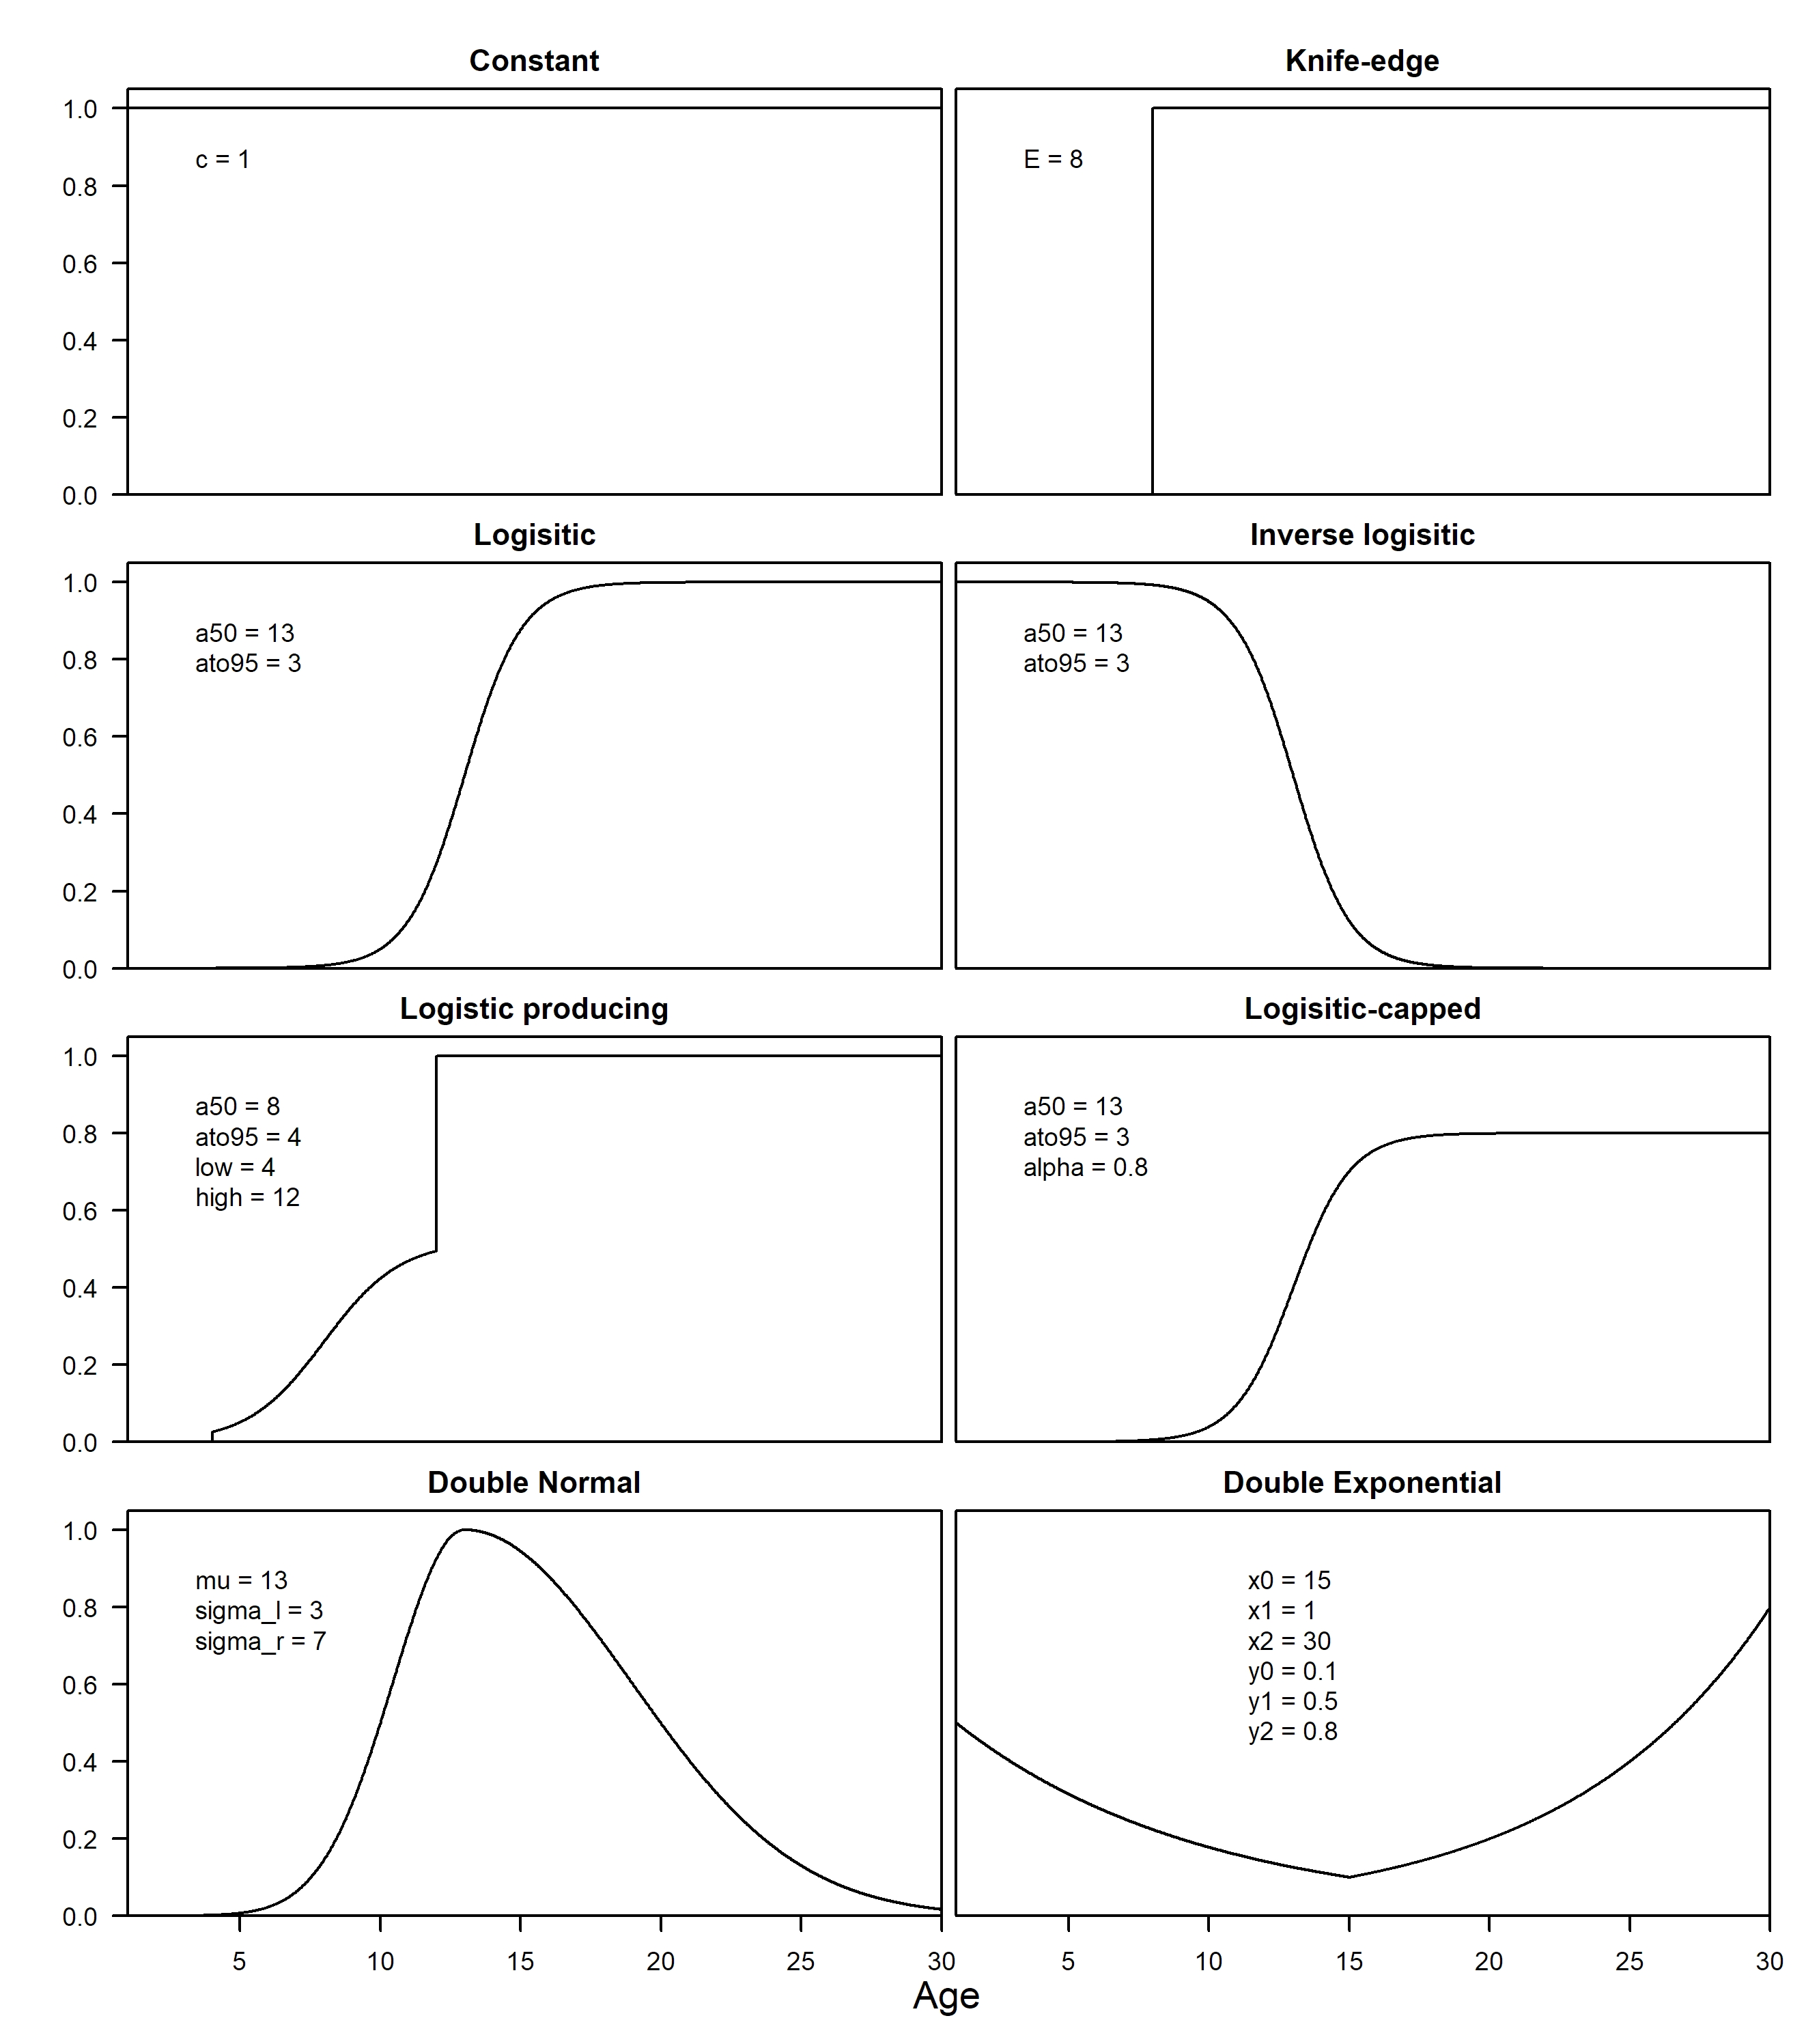
\includegraphics[scale = 0.9]{Figures/Selectivities.jpg}
	\caption{Examples of the selectivities}
	\label{fig:select examples}
\end{figure}

\subsection{\I{Time-varying parameters}}\label{sec:TimeVarying} \STATUS{Untested}

Any parameter can be varied annually for blocks of years or in specific years within the model run. For years that are not specified, the parameter will default to the input, or if in an iterative state such as estimation mode, the value being trialled at that iteration. The value used in the configuration file, input parameter file, or trialled value during estimation should be applied during initialisation phases.

Method types for a time-varying parameter are:

\begin{itemize}
\item \subcommand{constant},
\item \subcommand{exogenous},
\item \subcommand{linear},
\item \subcommand{annual\_shift},
\item \subcommand{random\_walk}, and
\item \subcommand{random\_draw}.
\end{itemize}

This option allows for a parameter to be fixed in a year, or be the result of a deterministic or stochastic process. Note that the stochastic time-varying methods (e.g., random\_walk and random\_draw) are intended for simulations or projections --- they should not be used in estimation as they utilise random numbers to generate parameter values. 

To implement a hierarchical model using the time-varying functionality, use MCMC estimation as a way to calculate the integral which is required to obtain unbiased estimates. Here, the prior parameter values need to be estimated using hyper-priors. In an MCMC context, a Gibbs sampler is assumed. That is, every draw is from a conditional distribution and so every draw is a candidate value.

When allowing time-varying parameters (such as in catchability coefficients or selectivities parameters), a model is given freedom to more closely match the observed data. Time-varying parameters can be used to allow the mean or shape parameters of selectivities to change between years, and potentially as a function of a linked variable.

An example of this is in the New Zealand hoki stock assessment where the $\mu$ and $a_{50}$ parameters are allowed to shift depending on when the fishing during the season occurs. Descriptive analysis showed that when fishing was earlier relative to other years, smaller fish were caught and vice versa. This can be shown in the Examples/2stock directory, implemented at line: \texttt{382} in the \texttt{population.csl2} file.

\subsubsection[Constant (year blocks)]{\argument{constant}}\index{Time-varying Parameters!Constant}\label{sec:TimeVarying-Constant}

This option allows a parameter to have an different value during specified years than the rest of the model run. This value can be estimated.

To allow survey catchability to be different in the year block 1975 to 1988 from the rest of the series we write:

{\small{\begin{verbatim}
		@time_varying q_time_var
		type          constant
		parameter     catchability[survey_q].q
		years         1975:1988
		values        0.001 # the same for all years
		\end{verbatim}}}

To estimate catchability for 1975 and 1976, use the following:

{\small{\begin{verbatim}
		@estimate q_time_var
		type uniform   #prior
		parameter time_varying[q_time_var].values{1975:1976}
		lower_bound 1e-6 1e-6
		upper_bound 2    2
		\end{verbatim}}}

To make the catchability be same over the year block we need to estimate it for one year (say 1975) and use the \textit{same} subcommand to make the others take the same value

{\small{\begin{verbatim}
		@estimate q_time_var
		type uniform
		parameter time_varying[q_time_var].values{1975}
		same      time_varying[q_time_var].values{1976:1988}
		lower_bound 1e-6
		upper_bound 2
		\end{verbatim}}}

\textbf{Caution}: do not estimate both the actual parameter and its time-varying counterpart, as the time-varying value will overwrite the actual parameter making the actual value unidentifiable. \TODO{this section required a re-write and clarification of the code and the text}

\subsubsection[Linear]{\argument{linear}}\index{Time-varying Parameters!Linear}\label{sec:TimeVarying-Linear}

Parameters are shifted based on a linear trend, with a given slope and intercept. An example of this is an exploitation selectivity parameters that may increase or decrease between years based a simple linear trend.

\begin{equation}
	\delta_y = a E_y + b
\end{equation}
\begin{equation}
	\theta'_y = \theta_y + \delta_y
\end{equation}

where $\delta_y$ is the shift or deviation in parameter $\theta_y$ in year $y$ to generate the new parameter value in year $y$ ($\theta'_y$). $a$ is an estimable slope parameter and $b$ is the linear trend intercept.

\subsubsection[Exogenous]{\argument{exogenous}}\index{Time-varying Parameters!Exogenous}\label{sec:TimeVarying-Exogenous}

Parameters are shifted based on an exogenous variable. An example of this is an exploitation selectivity parameters that may vary between years based on known changes in exploitation behaviour such as season, start time, and average depth of exploitation.

\begin{equation}
	\delta_y = a(E_y - \bar{E})
\end{equation}
\begin{equation}
	\theta'_y = \theta_y + \delta_y
\end{equation}

where $\delta_y$ is the shift or deviation in parameter $\theta_y$ in year $y$ to generate the new parameter value in year $y$ ($\theta'_y$). $a$ is an estimable shift parameter, $E$ is the exogenous variable, and $E_y$ is the value of this variable in year $y$. For more information readers can see \cite{francis_03}.

\subsubsection[Annual shift]{\argument{annual\_shift}}\index{Time-varying Parameters!Annual shift} \label{sec:TimeVarying-AnnualShift}

A parameter generated in year $y$ ($\theta'_y$) depends on the value specified by the user ($\theta_y$) along with three coefficients $a$, $b$, and $c$

\begin{equation}
	\bar{\theta}_y = \frac{\sum_{y}^Y\theta_y}{Y}
\end{equation}
\begin{equation}
	\theta'_y = a \bar{\theta}_y + b\bar{\theta}_y^{2} + c\bar{\theta}_y^{3}
\end{equation}

\subsubsection[Random Walk]{\argument{random\_walk}}\index{Time-varying Parameters!Random Walk}\label{sec:TimeVarying-RandomWalk}

A random deviate drawn from a standard normal distribution is added to the previous year's value. This option has an estimable parameter $\sigma_p$ for each time-varying parameter $p$. For reproducible modelling when using stochastic functionality, set the random seed (see Section~\ref{sec:CommandLineArguments}).

{\small{\begin{verbatim}
			@time_varying q_time_var
			type          random_walk
			parameter     catchability[survey_q].q
			distribution  normal
			mean          0
			sigma         3
\end{verbatim}}}

If the \texttt{parameter} specified in the \command{time\_varying} block is associated with an \command{estimate} block, then the parameter is constrained to stay within the lower and upper bounds of the \command{estimate} block.

\textbf{WARNING:} if the parameter does not have an associated \command{estimate} block then there is no safeguard against the application of a random deviate resulting in parameter values which cause the model to fail, i.e., generates NA or INF values. To avoid this, specify an \command{estimate} block even though the parameter is not actually being estimated; see the example syntax below.

A constraint whilst using this functionality is that a parameter cannot be less than 0.0. If it is then \CNAME\ sets it equal to 0.01.

{\small{\begin{verbatim}
			@estimate survey_q_est
			type      uniform
			parameter catchability[survey_q].q
			lower_bound 1e-6
			upper_bound 10
\end{verbatim}}}

This configuration will insure the random walk time-varying process will set the any new candidate values within the lower and upper bound of the \command{estimate} block.

\subsubsection[Random Draw]{\argument{random\_draw}}\index{Time-varying Parameters!Random Draw}\label{sec:TimeVarying-RandomDraw}

A random deviate drawn from a standard normal distribution used. This option has an estimable parameter $\sigma_p$ for each time-varying parameter $p$. For reproducible modelling when using stochastic functionality, set the random seed (see Section~\ref{sec:CommandLineArguments}).

{\small{\begin{verbatim}
			@time_varying q_time_var
			type          random_draw
			parameter     catchability[survey_q].q
			distribution  normal
			mean          0
			sigma         3
\end{verbatim}}}

If the \texttt{parameter} specified in the \command{time\_varying} block is associated with an \command{estimate} block, then the parameter is constrained to stay within the lower and upper bounds of the \command{estimate} block.

\textbf{WARNING:} if the parameter does not have an associated \command{estimate} block then there is no safeguard against the application of a random deviate resulting in parameter values which cause the model to fail, i.e., generates NA or INF values. To avoid this, specify an \command{estimate} block even though the parameter is not actually being estimated; see the example syntax below.

A constraint whilst using this functionality is that a parameter cannot be less than 0.0. If it is then \CNAME\ sets it equal to 0.01.

{\small{\begin{verbatim}
			@estimate survey_q_est
			type      uniform
			parameter catchability[survey_q].q
			lower_bound 1e-6
			upper_bound 10
\end{verbatim}}}

This configuration will insure the random draw time-varying process will set the any new candidate values within the lower and upper bound of the \command{estimate} block.

\subsection{\I{Equation parser}\label{sec:eq_parser}} \STATUS{Untested}

\CNAME\ has an equation parser, which is currently implemented in Projections (Section~\ref{sec:Project}), Derived quantities (Section~\ref{sec:DerivedQuantity}), and Reports (Section~\ref{sec:Report}).

Examples of syntax for implementing the equation parser are below. For more information on the parser, see \url{https://github.com/nickgammon/parser/blob/master/parser.cpp}

{\small{\begin{verbatim}
		equation process[Recruitment].r0 * 2 #double the recruitment
\end{verbatim}}}

mathematical functions such as \texttt{sqrt()}, \texttt{log()},  \texttt{exp()},  \texttt{cos()}, \texttt{sin()}, and \texttt{tan()} can be used

{\small{\begin{verbatim}
		equation sqrt(process[Recruitment].r0)
\end{verbatim}}}

exponents can be used with \texttt{pow()}

{\small{\begin{verbatim}
		equation pow(2, 3)
\end{verbatim}}}

the absolute value of an equation using \texttt{abs()}

{\small{\begin{verbatim}
		equation abs(sqrt(process[Recruitment].r0) * 1.33)
\end{verbatim}}}

\texttt{if-else} statements can be used

{\small{\begin{verbatim}
		equation if(process[Recruitment].r0 > 23, 44, 55)
		## if R0 is greater than 23 return 44 else return 55
\end{verbatim}}}

\texttt{if-else} statements can also be linked, more complex syntax

{\small{\begin{verbatim}
# if R0 > 23 return 44
# else if R0 < 23 & r0 > 10 return 55
equation if(process[Recruitment].r0 > 23, 44,
         if(process[Recruitment].r0 > 10, 55, 66))
else R0 must be less than 10 return 66
\end{verbatim}}}

Only single values can be referenced, so an equation cannot be applied to a vector, e.g., \subcommand{process[Recruit].recruitment\_multipliers\{1974:1980\}} cannot be referenced. More information on which parameters can be included in the equation parser is available (Section~\ref{sec:syntax}). Any subcommand that has a \texttt{type estimable} could be referenced with the equation parser.

\textbf{Note:} the equation parser will not catch all user configuration errors, such as checking whether a parameter that exists in the system has been populated when it is required.

For example, the wrong year could be misspecified in the case of removals in year $y$ which is based on the state of the population in year $y-1$

{\small{\begin{verbatim}
		parameter process[removals].catch
		year 2015
		equation derived_quantity[percent_b0].values{2020}
\end{verbatim}}}

This example is a valid equation but it will have nonsensical results, since a value for 2020 is to be calculated using values for 2015. Although the equation parser adds flexibility, it is easy to incorrectly specify equations.

\subsection{\I{Specifying projections}}\label{sec:Project} \STATUS{Untested}

Given a set of estimated parameter values from a \textit{-e} or a MCMC run,
the model can be projected. Projection years are after the model run years, and are defined in the \command{model} command block using the \subcommand{final\_projection\_year} subcommand, i.e., projection years are \subcommand{final\_year + 1} through to \subcommand{final\_projection\_year}.

Parameter values for the projected years can be specified in a stochastic way or fixed at some value (the default is the estimated value if the parameter is not time-varying) and these are specified in the \command{project} block,

{\small{\begin{verbatim}

@project Future_ycs  # label
type       lognormal_empirical  # which method to use
parameter  process[Recruitment].ycs_values
years      2012:2016
multiplier 1
... # any other parameters
\end{verbatim}}}

The subcommands \subcommand{years} and \subcommand{parameter} are common to all projection methods. Subcommand \subcommand{years} specifies the years to apply the new values to for the parameter in \subcommand{parameter}. Note that the years can be before the \textit{final\_year}, e.g., it is normal to vary the last few recruitment multipliers (YCS) in a projection run because they are usually poorly estimated or they have been set to 1.  The argument \argument{multiplier} is a constant which is multiplied with the projected value after it has been generated. The \subcommand{type} subcommand gives the method to use to generate new parameter values.

\CNAME\ allows any estimable parameter to be specified in a \command{project} block and then varied from the estimated value in a projection. The available projection types for these parameters include:

\begin{itemize}
	\item constant
	\item lognormal
	\item empirical-lognormal
	\item empirical re-sampling
	\item user-defined
\end{itemize}

\CNAME\ has no default projection properties for parameters that are specified by year, e.g., recruitment multiplier parameters, time-varying parameters, and as a special case, future catches. For these, projections  must have a \command{project} command block. For example, \CNAME\ will produce errors if run in projection mode without a \command{project} block for the \subcommand{recruitment\_multipliers} parameter being specified.

DEPRECATED: \textbf{Note for the year class parameters:} the definition of year applies to the \argument{ycs\_years}, not the model years. As defined in Section \ifAgeBased \ref{sec:Process-RecruitmentBevertonHolt}\else \ref{sec:Process-RecruitmentBevertonHolt}\fi, \argument{ycs\_years} are offset between the time of spawning and when individuals are added to the partition.

Future catches are also specified in a \command{project} block, one for each fishery (see \ref{sec:Project-Catch} for examples). Here, a fishery is reference in the \textit{parameter} subcommand with the \textit{method\_} fragment to identify it,

 \textit{process[block label].method\_$[$fisheries label$]$},

For a process called \textit{Fishing} that has three fisheries defined, it would be \textit{process[Fishing].method\_pot} to specify the fishery labelled \textit{pot}.

The \CNAME\ command to run the model in projection mode is \texttt{Casal2 -f 1}. This functionality allows for the exploration of many scenarios with a single set of parameters. The number of projections should be greater than 1 only if applying a projection type that is stochastic.

The \texttt{-{}-tabular} flag should be used when running projections after a Bayesian analysis. This option will output a tabular report (see Section~\ref{sec:Tabular}) which can then be analysed in \R.

An example of the command line evocation is

\textit{casal2 -f 1 -i mcmc.txt --tabular $>$ projection.out.txt}

where \textit{mcmc.txt} is output from a MCMC run, one parameter set per row, which will give one projection per row, and \textit{projection.out.txt} will contain one row for each MCMC run in each of the reports specified in (usually) the \textit{Report.csl2} file (quantities as specified in the \textit{Report.csl2} file).

For a projection run in \CNAME, the model is initialised and run through the model years from \argument{start\_year} to \argument{final\_year}. During this run mode \CNAME\ stores all parameter values so that projection classes can allow parameters before \subcommand{final\_year} to be projected. The model then is re-run from \argument{start\_year} to \argument{projection\_final\_year}, where any parameter can either be fixed or drawn from a stochastic distribution or process.


\subsubsection{\I{Projection methods}\label{sec:ProjectionMethods}}

This section lists all the projections classes available, their functionality, and an example of the syntax.

\paragraph[Constant]{The constant projection type, \argument{constant}}\index{Projections!Constant}\label{sec:Project-Constant}

A parameter can either be fixed during all projection years or specified individually for each projection year. This is a deterministic assumption, where the parameter is assumed to be known without error during projection years.

{\small{\begin{verbatim}
		@project Future_ycs
		type      constant
		parameter process[Recruitment].recruitment_multipliers
		years     2012:2016
		values    1 2 1 2 0.5  # "values 3" means all years use 3
		multiplier 1
		\end{verbatim}}}


\paragraph[Multiple Values]{The multiple values projection type, \argument{multiple\_values}}\index{Project-MultipleValues}\label{sec:Project-MultipleValues}

Users can specify a set of values for each projection year for each row in the \texttt{-i} or \texttt{-I} file using the \subcommand{multiple\_values} projection class. This gives users flexibility in specifying a range of bespoke values during projections and including uncertainty in the projected values. See below for an example on how to configure this class.

{\small{\begin{verbatim}
@project future_disease_rates
type multiple_values
parameter process[dtransition].proportions{disease}  
years 2024:2026
table values
2024 2025 2026
0.1 0.2 0.3
0.3 0.4 0.5
end_table
\end{verbatim}}}

\paragraph[Empirical sampling]{Sampling from a range of years, type  \argument{empirical\_sampling}}\index{Projections!Empirical sampling}\label{sec:Project-EmpiricalSampling}

Parameters that have time components associated with them can be sampled uniformly with replacement over a range of years and used as values for the projected years. The year range to sample from is between \argument{start\_year} and \argument{final\_year}:

{\small{\begin{verbatim}
		@project   Future_ycs
		type       empirical_sampling
		parameter  process[Recruitment].standardised_recruitment_multipliers
		years     2012:2016
		start_year 1988     # re-sample from estimated values
		final_year 2008     # from 1988 to 2008 inclusive
		multiplier 1
		\end{verbatim}}}

Note that when projecting recruitment\_multipliers, the \emph{unstandardised} values are used. This may cause projections to be other than what was intended unless these average one (or some other chosen value). If not using a transformation (e.g., the simplex transformation for recruitments), a vector average penalty should be applied (and the resulting recruitment multipliers checked) to ensure the average recruitment multiplier is equal to one over some pre-defined range. 

\paragraph[Lognormal]{Sampling from a Lognormal distribution, type  \argument{lognormal}}\index{Projections!Lognormal}\label{sec:Project-LogNormal} \STATUS{Untested}

The parameters are drawn from a Gaussian (Normal) distribution in log space and exponentiated  to result in the Lognormal distribution

\begin{equation}\label{eq:lognormal}
X_p = exp(\epsilon_p - \sigma^2 / 2)
\end{equation}

where $\epsilon_p\stackrel{iid}{\sim}N(\mu,\sigma)$ and $X_p$ is the projected value for parameter $X$, and $\mu$ and $\sigma$ are the mean and standard deviation on the log scale.

An example of applying this process to draw future year class parameters from a Lognormal distribution with mean 1 and standard deviation 0.8

{\small{\begin{verbatim}
		@project Future_ycs
		type     lognormal
		parameter process[Recruitment].recruitment_multipliers
		years     2012:2016
		mean      0     # mean 1 on un-transformed scale
		sigma     0.8   # log scale
		multiplier 1
		\end{verbatim}}}

\paragraph[Lognormal-Empirical]{Sampling from a Lognormal distribution where the  variance is estimated from values over a specified year range, type  \argument{lognormal\_empirical} }\index{Projections!Lognormal-Empirical}\label{sec:Project-LogNormalEmpirical} \STATUS{Untested}

This method applies a Lognormal draw as in the \argument{Lognormal} method above and specifies a year range from which the standard deviation of the distribution is calculated. Then equation~\eqref{eq:lognormal} is used to generate future values with a specified $\mu$ and empirically calculated $\sigma$,

{\small{\begin{verbatim}
		@project Future_ycs
		type      lognormal_empirical
		parameter process[Recruitment].recruitment_multipliers
		years     2012:2016
		mean      0
		start_year 1988   # range of years to take the
		final_year 2008   # values for \math{\sigma}
		multiplier 1
		\end{verbatim}}}

%\paragraph[User Defined]{Sample from a user-defined function, \argument{user\_defined}}\index{Projections!User Defined}\label{sec:Project-UserDefined} \STATUS{Untested}

%This method uses the equation parser to calculate the values to use in the projection. This was set up to define and apply harvest control rules (e.g., apply a management action such as changing catch limits based on the current or previous state).

%In fisheries models, this option can be used to calculate the projected catch based on an exploitation rate multiplied by the vulnerable biomass, where the exploitation rate is based on a rule (Figure~\ref{fig:HCR}).

%\begin{figure}[!h]
%	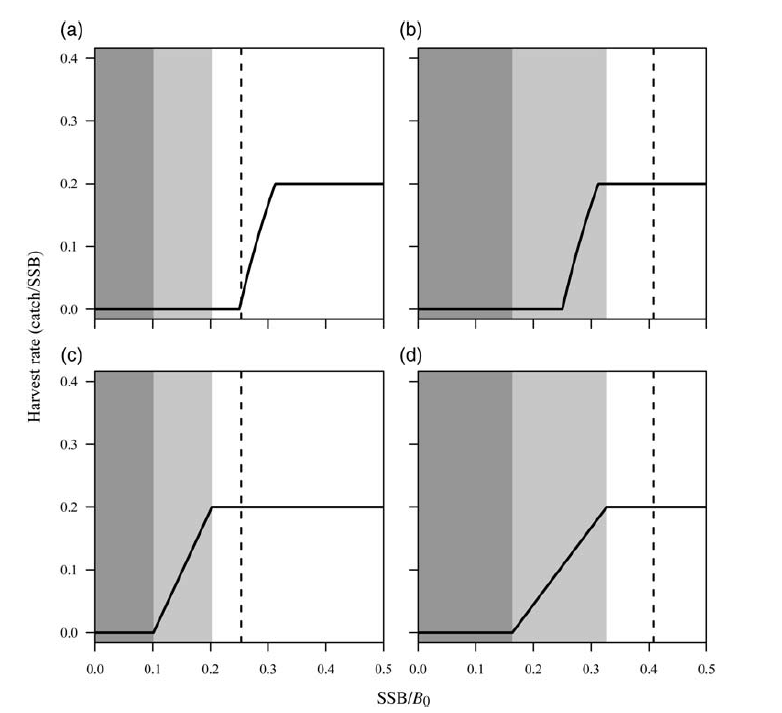
\includegraphics[scale=0.9]{Figures/HarvestControlRules.png}
%	\caption{\textbf{Examples of control rules based on current stock status.}}
%	\label{fig:HCR}
%\end{figure}

%\pagebreak
%{\small{\begin{verbatim}
%		@project HCR_2015
%		type       user_defined
%		parameter process[Instantaneous_Mortality].method_Sub_Ant_F
%		years 2015
%		equation if(derived_quantity[SSB].values{2014} / process[Recruitment].b0 <= 0.1, 0.0,
%		if(derived_quantity[SSB].values{2014} / process[Recruitment].b0 > 0.1 &&
%		derived_quantity[SSB].values{2014} / process[Recruitment].b0 < 0.2,
%		derived_quantity[SSB].values{2014} * derived_quantity[SSB].values{2014}
%		/ process[Recruitment].b0,
%		derived_quantity[SSB].values{2014} * 0.2))
%		\end{verbatim}}}

%Care should be taken when writing user-defined equations. The above equation is: if $\%B_{2014} \leq 0.1$ then set next year's catch to 0.0, else if $\%B_{2014} > 0.1 \text{ } \& \text{ } \%B_{2014} \leq 0.2$ then set next year's catch equal to $\%B_{2014} \times SSB_{2014}$, else set next year's catch to $0.2 SSB_{2014}$.

\paragraph[Catches]{Specifying catch for projections }\index{Projections!Catches}\label{sec:Project-Catch}

Catches are unique in that they are known inputs in a table format. For example, to project catches that are in a table

{\small{\begin{verbatim}
# fishing process
@process Fishing
type mortality_instantaneous_retained
m 0.17*6
time_step_proportions 1
relative_m_by_age One*6   # For age based model. 
                          # For length-based models use relative_m_by_length
categories *
table catches
year\begin{center}
	\begin{center}
		
	\end{center}
\end{center}
hingPot	Recreation
1900	0	0	0
1901	13.2	0	22.9
1902	26.4	0	23.5
1903	39.6	0	24
end_table

# projection block
@project future_catch
type      constant
parameter process[Fishing].method_fishingpot
years     2020:2029
values    4000
\end{verbatim}}}

This uses the syntax \texttt{block\_type[block\_label].method\_fishinglabel}. \textbf{Note:} the fishing label which is defined in the table needs to be lower case form in the \command{projection} block. Notice the use of \textit{method\_} syntax to identify the right fishery.
